\documentclass[11pt]{article}

\usepackage[french]{babel}

\usepackage[T1]{fontenc}
\usepackage{float}

\usepackage{amsfonts}
\usepackage{amsmath}
\usepackage{amssymb}

\usepackage{graphicx}
\usepackage{multirow}
\usepackage{multicol}
\usepackage[dvipsnames]{xcolor}
\usepackage[colorlinks=true, allcolors=black]{hyperref}
\usepackage{hyperref}

\usepackage{mathtools}
\usepackage{siunitx}
\usepackage{physics}

\usepackage{listings}
\usepackage{tikz}


\usepackage{caption}
\usepackage{subcaption}

\usepackage[
    backend=biber, 
    natbib=true,
    style=ieee,
    sorting=none
]{biblatex}

\newpage
\usepackage[left=2.5cm,top=3cm,right=2.5cm,bottom=3cm,bindingoffset=0.5cm]{geometry}


\bibliography{bibliography.bib}

 
\begin{document}
\begin{titlepage}
    \begin{center}
        {\fontsize{20}{40} \selectfont \bfseries BSQ201 - Projet 2} \\\vspace{20pt} {\fontsize{20}{40} \selectfont \bfseries Optimisation du placement de cloches de dons de vêtements dans Sherbrooke}
        \\\vspace{120pt}
        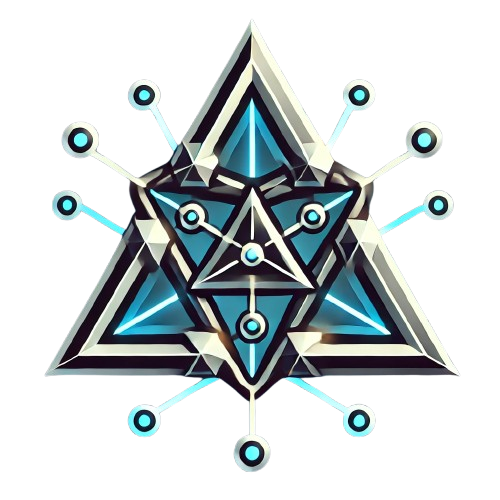
\includegraphics[width=0.3\textwidth]{images/QLink_noback.png} 
        \\\vspace{10pt}
        \textbf{ Ludovic Marcotte  \\\vspace{8pt}
        Sahar Saoudi\\\vspace{8pt} Louis-Félix Vigneux\\\vspace{8pt}}
        \vspace{100pt}
        \today
        \vfill
        \begin{figure}[h]
             \centering
             \begin{subfigure}[b]{0.3\textwidth}
                 \centering
                 
\includegraphics[width=\textwidth]{images/recupex_logo.png}
             \end{subfigure}
             \hfill
             \begin{subfigure}[b]{0.3\textwidth}
                 \centering
                 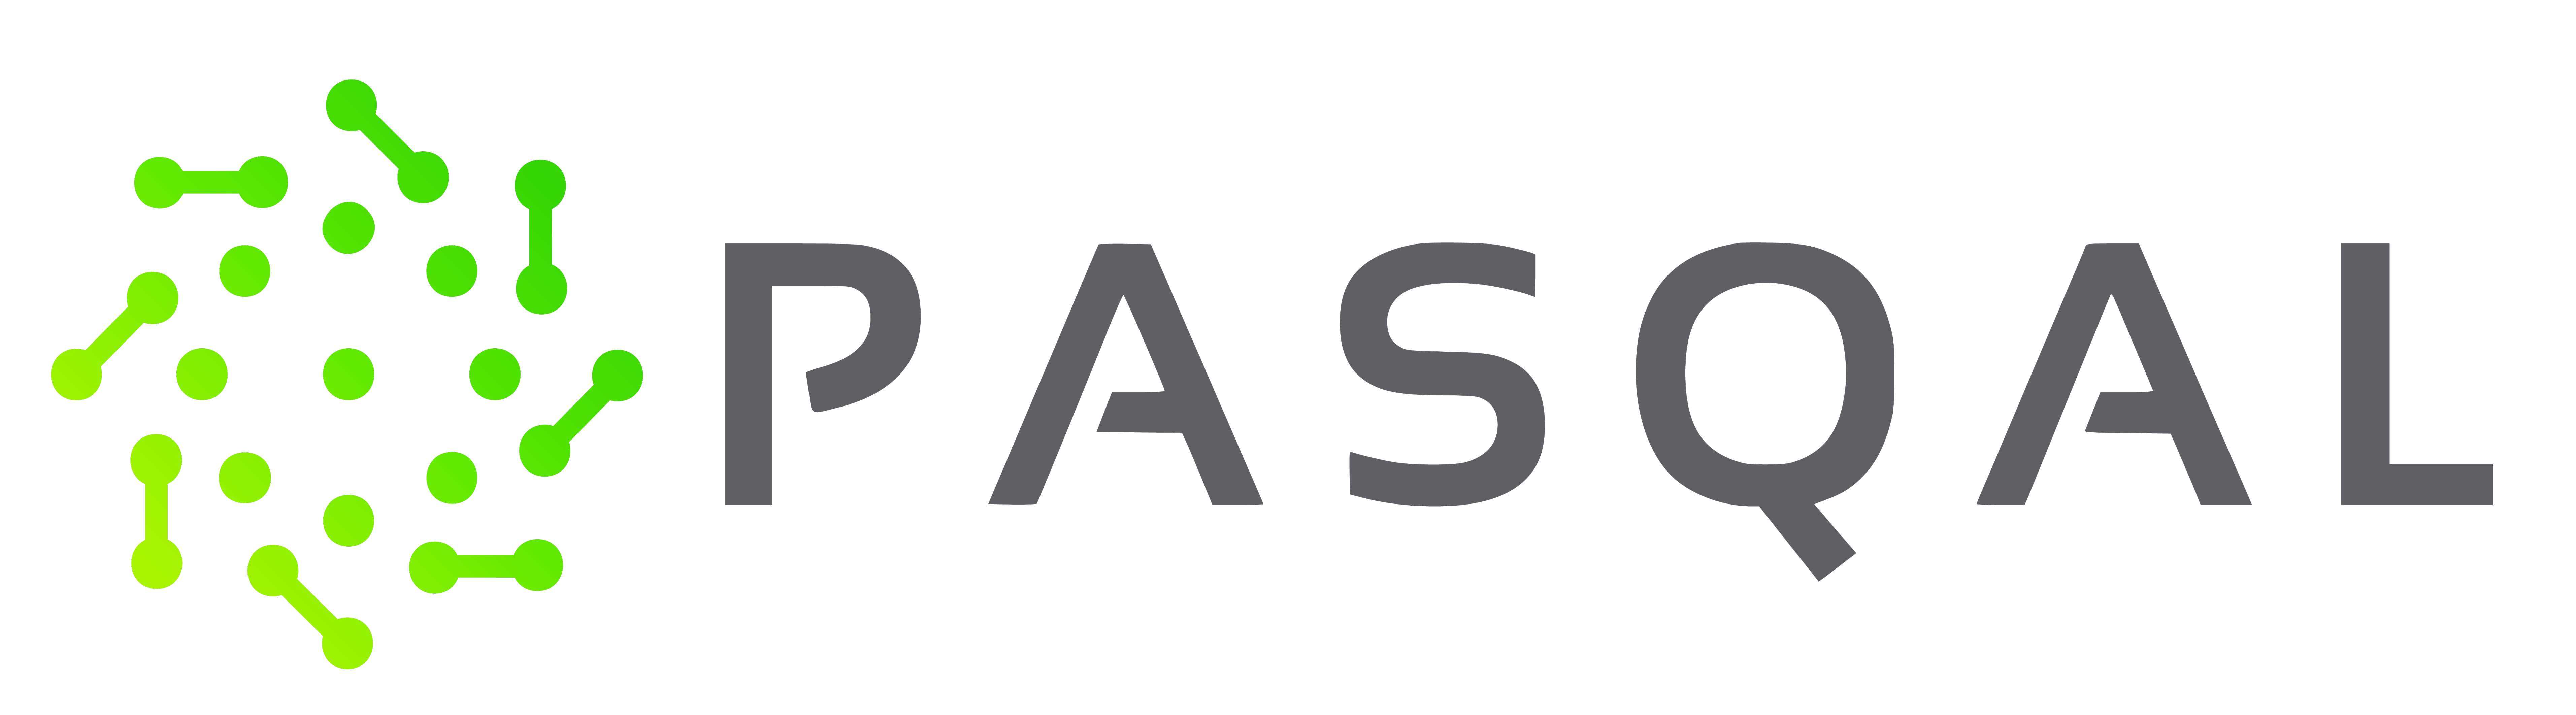
\includegraphics[width=\textwidth]{images/pasqal_logo.png}
             \end{subfigure}
             \hfill
             \begin{subfigure}[b]{0.3\textwidth}
                 \centering
                 
\includegraphics[width=\textwidth]{images/UdeS_logo_rgbHR.png}
             \end{subfigure}
        \end{figure}
    \end{center}
\end{titlepage}

\tableofcontents
\newpage
\section*{Abstract}
Nous proposons un algorithme adiabatique quantique (QAA) et d'optimisation approximative quantique (QAOA). Leur performace seront comparé à l'implémentation classique actuelle fournie dans la libraire \textit{networkx} en python. L'algorithme adiabatique et classique permettra de régler la problématique de Récupex consistant à replacer leur cloches récoltant les vêtements usagers dans une distribution optimial pour couvrir le territoire de la ville de Sherbrooke, Québec, Canada. Une recombinaison déterministe pour trouver une approximation d'un ensemble indépendant maximal à l'aide de sous-graphes est aussi présentée. Finalement, il sera déterminé s'il est pertinent actuellement ou dans un futur proche d'envisager les mtéthodes quantiques analogues pour résoudre ce problème.

\section{Introduction}
Récupex est un organisme à but non lucratif dédié à l’insertion socioprofessionnelle des personnes en difficulté d’employabilité. L’organisme gère un vaste réseau de collecte de vêtements, avec une centaine de bacs répartis principalement à Sherbrooke et dans la région de l’Estrie. En partenariat avec des friperies et d’autres organismes communautaires, Récupex contribue activement à la valorisation des textiles usagés, sensibilisant la population aux enjeux environnementaux et recyclant environ 3,5 millions de livres de textiles chaque année.

La gestion des bacs de récupération de vêtements à Sherbrooke présente des défis importants pour Récupex. Les performances varient selon les emplacements en termes de volume de dons, de qualité des textiles et de nuisances (dépôts sauvages, vandalisme). La logistique de collecte demande des ressources significatives (chauffeurs, camions, matériel), rendant l'entretien complexe. Récupex cherche donc à optimiser l'emplacement de ses bacs pour améliorer la collecte, minimiser les nuisances et assurer une gestion efficace des ressources.

\section{Objectifs}
- Aider l'organisation Récupex à ameliorer leur gestion de bacs de récuperation en utilisant différents approches quantiques (QAA et QAOA).
- Évaluer à quel point les approches quantiques sont pertinentes comparées aux méthodes classiques.
- Répondre aux conditions de recupex mentionnées dans la sous-section suivante.

\subsection{Conditions d'évaluation des cloches de don de Récupex}
Récupex applique plusieurs critères pour optimiser l’emplacement de ses bacs de récupération de vêtements, en tenant compte des aspects de couverture, d'accessibilité, et de performance :

\begin{enumerate}
    \item \textbf{Couverture des territoires non desservis} : Récupex cherche à s’assurer que chaque région a accès à un bac, en priorisant les territoires non encore desservis. Cela vise à améliorer l’accessibilité pour tous.

    \item \textbf{Proximité et accessibilité} : Plus un bac est proche des habitants, plus il est accessible et utilisé. Récupex souhaite donc placer les bacs dans des zones faciles d’accès pour maximiser la collecte.

    \item \textbf{Contrôle de la densité de bacs} : Bien qu’il soit important d’avoir des bacs à proximité, Récupex évite de multiplier les bacs dans la même zone pour éviter la redondance et les coûts inutiles.

    \item\textbf{Qualité des dons} : La qualité des vêtements collectés varie selon les quartiers. Dans les zones plus aisées, les vêtements ont tendance à être de meilleure qualité. Cela peut influencer le placement des bacs en fonction des priorités de collecte de qualité.

    \item\textbf{Densité de population} : Les secteurs densément peuplés sont plus propices à accueillir plusieurs bacs, car ils génèrent un volume de dons plus élevé.

    \item\textbf{Pertinence et fonctionnalité des bacs} : Récupex suit la performance de chaque bac (s’il est régulièrement utilisé ou non) pour ajuster leur distribution, en ajoutant, déplaçant ou retirant des bacs selon leur pertinence dans chaque zone.

    \item\textbf{Prendre en consideration les autres associations} : Récupex prend en compte la présence d’autres associations, comme Estrie Aide, pour éviter une concurrence directe et mieux répartir les services.

    \item\textbf{Autorisation pour le placement} : Le placement de chaque bac nécessite une autorisation, et il est plus facile d’obtenir cette autorisation dans des zones où les propriétaires ouverts au projet.
\end{enumerate}

\section{Théorie}
\subsection{Graphes}
\subsubsection{Introduction aux graphes}
Un graphe est un objet mathématique très utile lorsqu'une carte doit être représentée dans un ordinateur \cite{mackaness_use_1993}\cite{riaz_applications_2011}. Ce dernier est représenté par un ensemble $G=(V,E)$ où V est un ensemble de sommets et E l'ensemble des arrêtes du graphe. Un sommet est un point dans l'espace qui sera connecté à un autre grâce à une arrête. Voici la manière usuelle de représenter un graphe.

\begin{figure}[H]
    \centering
        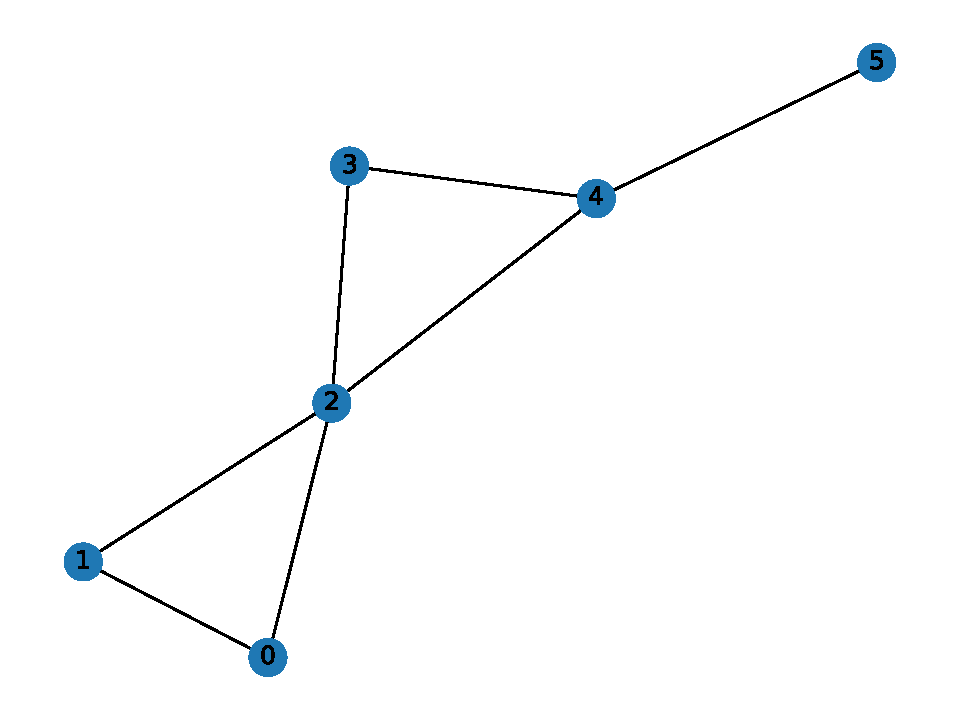
\includegraphics[width=0.45\linewidth]{images/graphe_MIS_exemple.pdf}
        \caption{Exemple de graphe}
    \label{graph_exemple}
\end{figure}

Par contre, l'utilisation de graphes par disques unitaires sera plus approprié pour le projet. Dans ce type de graphe, on note la position des sommets dans l'espace et non leur relation entre eux. Pour définir les opérations, nous traçons un disque de rayon arbitrairement défini plutôt auparavant. Ensuite, si deux cercles de deux sommets distincts se croisent, il y a alors une interaction entre ces deux sommets. Voici la comparaison entre un graphe de disque unitaire et son analogue de représentation plus «classique».  \textbf{Inclure image d'un graphe de disque vs son graphe}

\subsubsection{Ensemble indépendant maximal}
Un ensemble indépendant maximal est un ensemble de sommets qui ne sont pas connectés par une arête. Cet ensemble doit contenir le plus de sommets possible afin d'être complet. Par exemple, le graphe de la figure 1 comporte 6 noeuds et son ensemble indépendant maximal en comporte 3.
 
Il peut y avoir plusieurs ensembles indépendants maximaux pour un seul graphe comme c'est le cas avec le graphe précédant. Les ensembles correspondants seraient {1, 4, 6} et {2, 4, 6} comme illustré par la figure 2.

\begin{figure}[H]
    \centering
    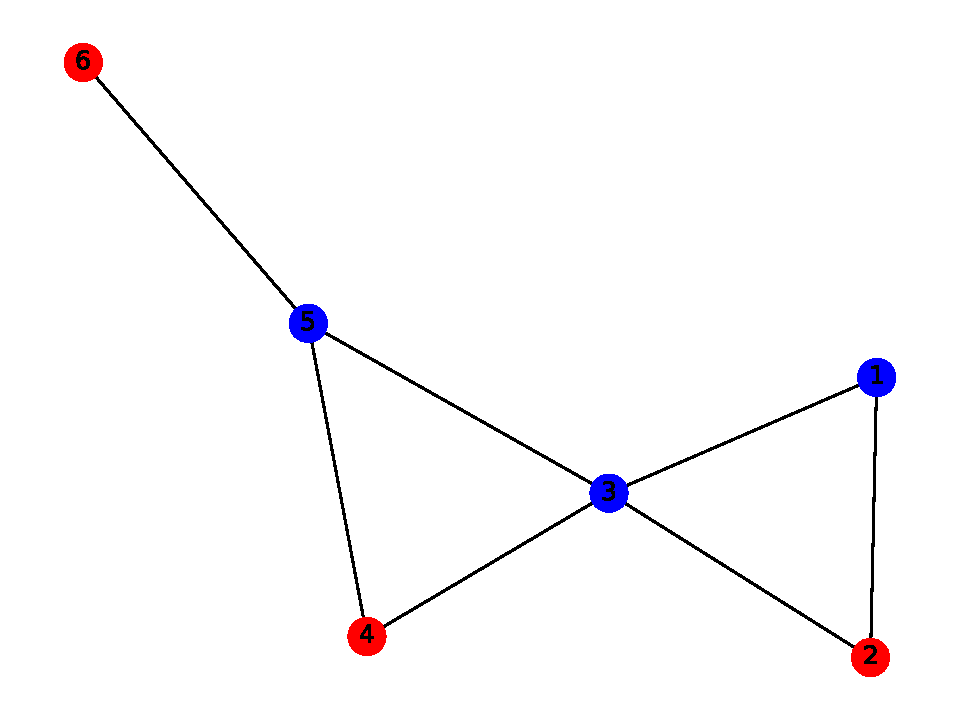
\includegraphics[width=0.4\linewidth]{images/graphe_MIS_1.pdf}
    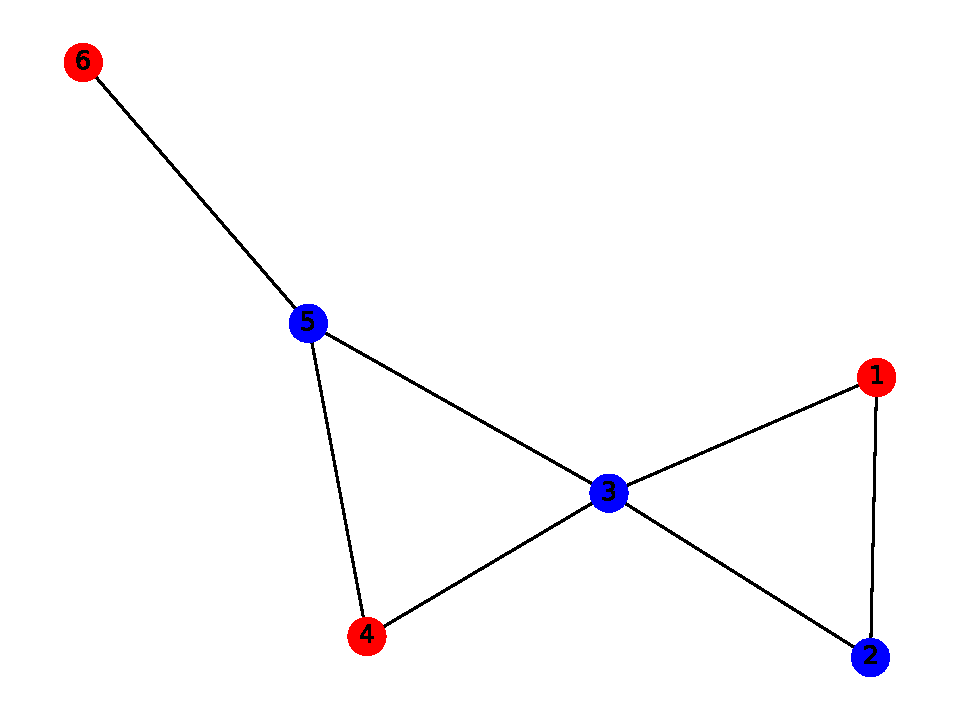
\includegraphics[width=0.4\linewidth]{images/graphe_MIS_2.pdf}
    \caption{Ensembles indépendants maximals pour le graphe de la figure 1.}
    \label{MIS_exemple}
\end{figure}



\subsection{Grapher sherbrooke}
Récupex se doit de couvrir l'ensemble de Sherbrooke au meilleur de ses possibilité avec ses 60 bacs. Il faut alors trouver une manière de représenter la ville dans l'ordinateur quantique. Pour ce faire,  nous allons utiliser un graphe. 

Pour utiliser cet objet mathématique dans notre problématique, nous allons représenter tout les emplacement possible des bacs par un sommet du graphe. Ces emplacements ont été définis grâce à une base de données des édifices commerciaux et indutriels de la ville de Sherbrooke \cite{noauthor_repertoire_nodate}. Nous avons raffiné cette base de données en gardent seulement les commerces, les institutions et lieux publics. En effet, les bacs ne peuvent pas placé sur un terrain résidentiel ou industriel pour encourager les dons. Nous allons représenter le graphe de la ville selon un graphe de disque unitaire. Les sommets du graphe sont donc ces emplacements possibles et nous nottons leur position dans l'espace par leur longitude sur l'axe des x et leur latitude sur l'axe des y. Par la suite, pour définir les arrêtes du graphes, il suffit de définir un rayon pour lequelles les endroits possibles sont connectés. Par la suite, un algorithme d'ensemble indépendant maximal pourra être utilisé pour faire ressortir le nombre maximal d'emplacments qui ne sont pas trop proches des autres pour mettre des bacs.

Puisque les ordinateurs quantique utilisé dans ce projet ont une limite de 25 atomes, nous devons alors simplifier ces graphes. Pour ce faire, nous avons utiliser un algorithme d'ensemble indépendant maximal classique pour réduire le nombre de données d'environ 3000 à 125 en utilisant un rayon de 1km. Cette opération crée déjà un pré-tri des endroits possibles en retirant des emplacements déjà trop près l'un de l'autre. Voici la simplification sous forme d'image. 

 \begin{figure}[H]
    \centering
        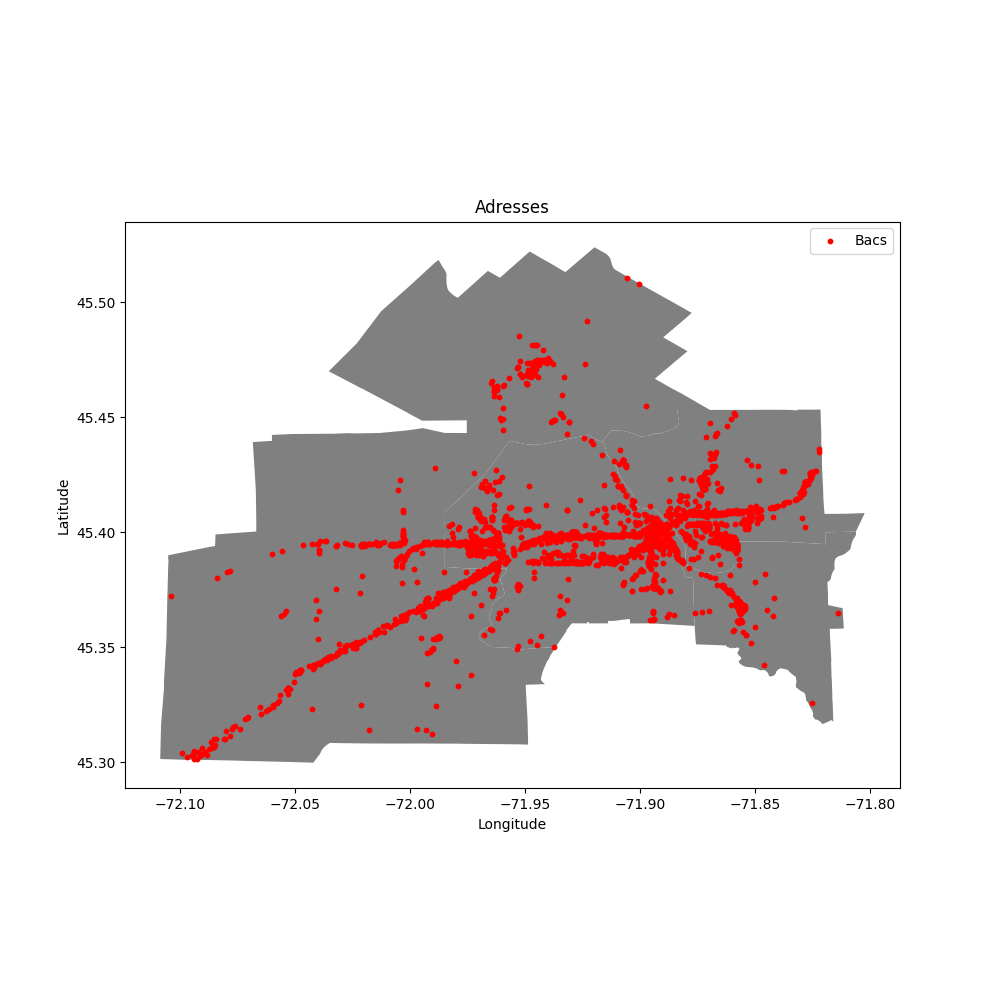
\includegraphics[width=0.5\linewidth]{images/commerces.png}
        \caption{Emplacements possibles des bacs dans la ville de Sherbrooke}
    \label{bacs_possibles_total}
\end{figure}


Cette carte de simplification sera utilisée pour le reste des calculs.

\subsection{Ordinateur quantique à atome neutre}
L'ordinateur quantique à atome neutre est un ordinateur quantique analogique. Les calculs nécessitent des manipulations afin d'être effectués. Pour ce projet, nous utiliserons les appareils développés par Pasqal \cite{browaeys_quantum_2019}. La première étape est de créer un registre contenant des atomes à certaines positions afin de représenter notre problème dans l'ordinateur. Pour ce projet, nous ne considèreront seulement que des registres en deux dimension. Des pinces optiques sont positionnées \cite{browaeys_pinces_2016} aux endroits déterminés afin de capturer les atomes. Puisque le taux de capture des pinces optiques est d'environ 50\%, le double du nombre de pinces optiques sont placés dans le registre. Après la capture des atomes, on vérifie la position des atomes capturés et les atomes sont replacés un à un afin de créer le registre voulu. Tout ce processus est fait directement par Pulser \cite{silverio_pulser_2022} lors de la création d'un registre. Le calcul quantique se fait à l'aide d'un pulse. Le pulse peut avoir plusieurs formes et atteint une certaine valeur maximale $\Omega_{max} $ qui définie le rayon de blocage. Le rayon de blocage définit un cercle autour des atomes du registre. Les atomes se tenant à l'intérieur de ce cercle demandent un pulse beaucoup plus grand afin de s'exciter. Une autre valeur importante pour le pulse est le désaccord. Le désaccord est une valeur qui influe sur le pulse envoyé. Un désaccord négatif pousse les atomes dans l'état fondamental alors qu'un désaccord positif pousse les atomes dans l'état excité. Durant le pulse, certains atomes vont s'exciter et seront alors éjectés du registre. On mesure donc par fuorescence les atomes dans l'état fondamental présents dans le registre à la suite du pulse pour déduire que les atomes manquants sont les atomes qui ont été excités. Cette mesure est aussi effectuée par Pulser directement. Ainsi, pour utiliser l'ordinateur quantique à atome neutre de Pasqal, l'utilisateur doit simplement définir une séquence contenant la forme du registre et le Pulse en fonction du temps. 


\subsection{Trouver l'ensemble indépendant maximal à l'aide de l'ordinateur quantique à atome neutre}
Maintenant que nous savons utiliser l'ordinateur quantique à atome neutre, nous allons résoudre le problème np complet \cite{tarjan_finding_1977} qu'est de trouver l'ensemble maximal indépendant d'un graphe géométrique \cite{dettmann_random_2016}. Deux méthodes s'offrent à nous, l'algorithme quantique adiabatique ou bien l'algorithme d'optimisation approximative quantique \cite{ebadi_quantum_2022}.

\subsubsection{Algorithme quantique adiabatique}
La première étape est de créer le registre en fonction du graphe. La clé est de ne considérer que les interractions entre les noeuds du graphe. Ces interractions sont reliées directement au rayon de blocage dans le registre. On doit alors positionner les atomes afin que s'il devrait y avoir une arête entre le deux atomes, les atomes sont couverts par le rayon de blocage de l'autre atome. Il ne reste plus qu'à construire un pulse avec une valeur de $\Omega_{max}$ en fonction du rayon de blocage souhaité comme en exemple à la figure 5.
\begin{figure}[H]
    \centering
    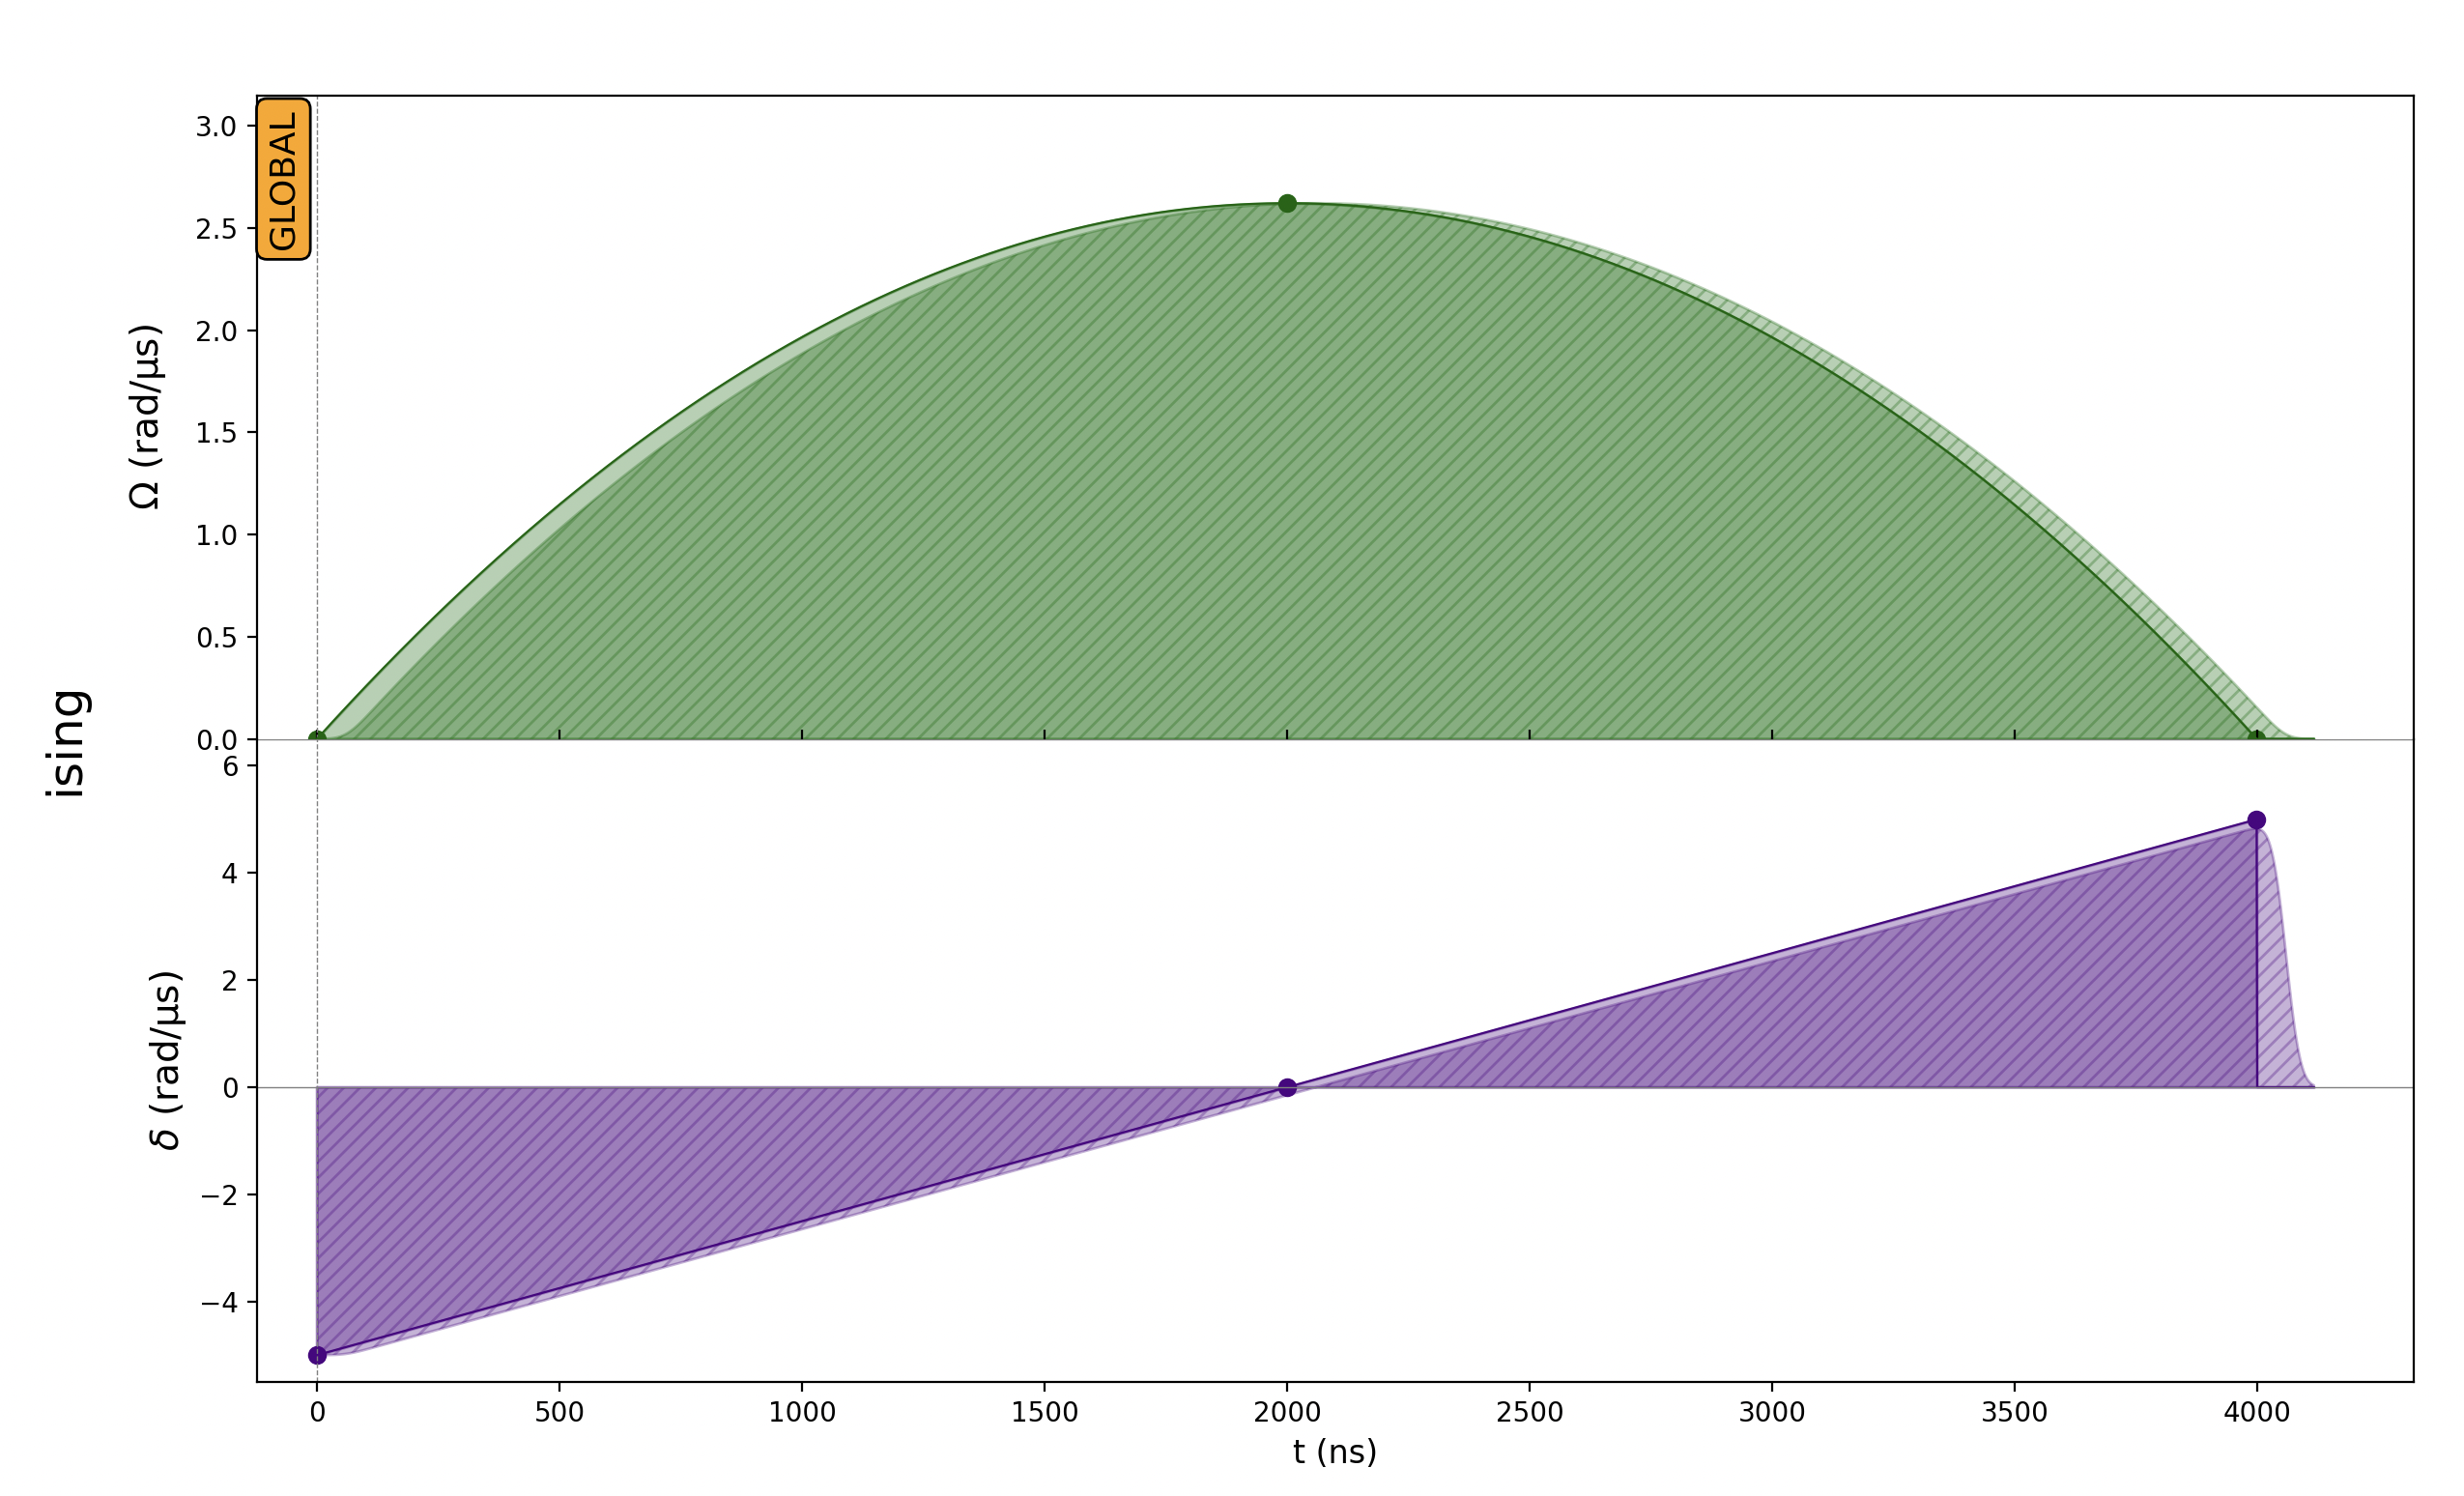
\includegraphics[width = 0.6\linewidth]{images/pulse_exemple.png}
    \caption{Exemple de Pulse adiabatique}
    \label{pulse_exemple}
\end{figure}
L'algorithme quantique adiabatique tente de transformer un hamiltonien initial en un hamiltonien final en lui appliquant le pulse pendant le plus de temps possible. L'hamiltonien initial du système est ici représenté par le registre initial que l'on crée. En lui appliquant le Pulse pendant assez longtemps, on trouve notre hamiltonien final qui encode la solution. En fait, on a vu que le rayon de blocage va empêcher les atomes qui sont dans ce rayon de s'exciter. Puisque les noeuds qui sont liés par une arête sont contenus dans le rayon de blocage, un seul des deux va pouvoir s'exciter. Ainsi, notre hamiltonien final ne contiendra que des atomes excités qui forment un ensemble indépendant maximal. Le calcul quantique ne donne pas toujours le même résultat et ne donne pas toujours l'ensemble indépendant maximal. En fait, puisque nous sommes limité par le temps durant lequel nous pouvons appliquer le pulse. Nous n'obtenons pas la meilleure réponse à chaque fois. Si le pulse pouvait s'appliquer beaucoup plus longtemps, il nous faudrait théoriquement un seul calcul pour trouver directement l'ensemble indépendant maximal par le théroème adiabatique \cite{amin_consistency_2009}. On effectue donc le calcul un certain nombre de fois afin d'obtenir un histogramme contenant plusieurs résultats. Les résultats qui sortent le plus souvent dans l'histogramme sont des ensembles maximals indépendants. Par exemple, on pourrait prendre le graphe de la figure 1 et trouver l'ensemble indépendant maximal avec les étapes expliquées ci-dessus afin d'obtenir le registre et l'histogramme de la figure 6.
\begin{figure}[H]
    \centering
    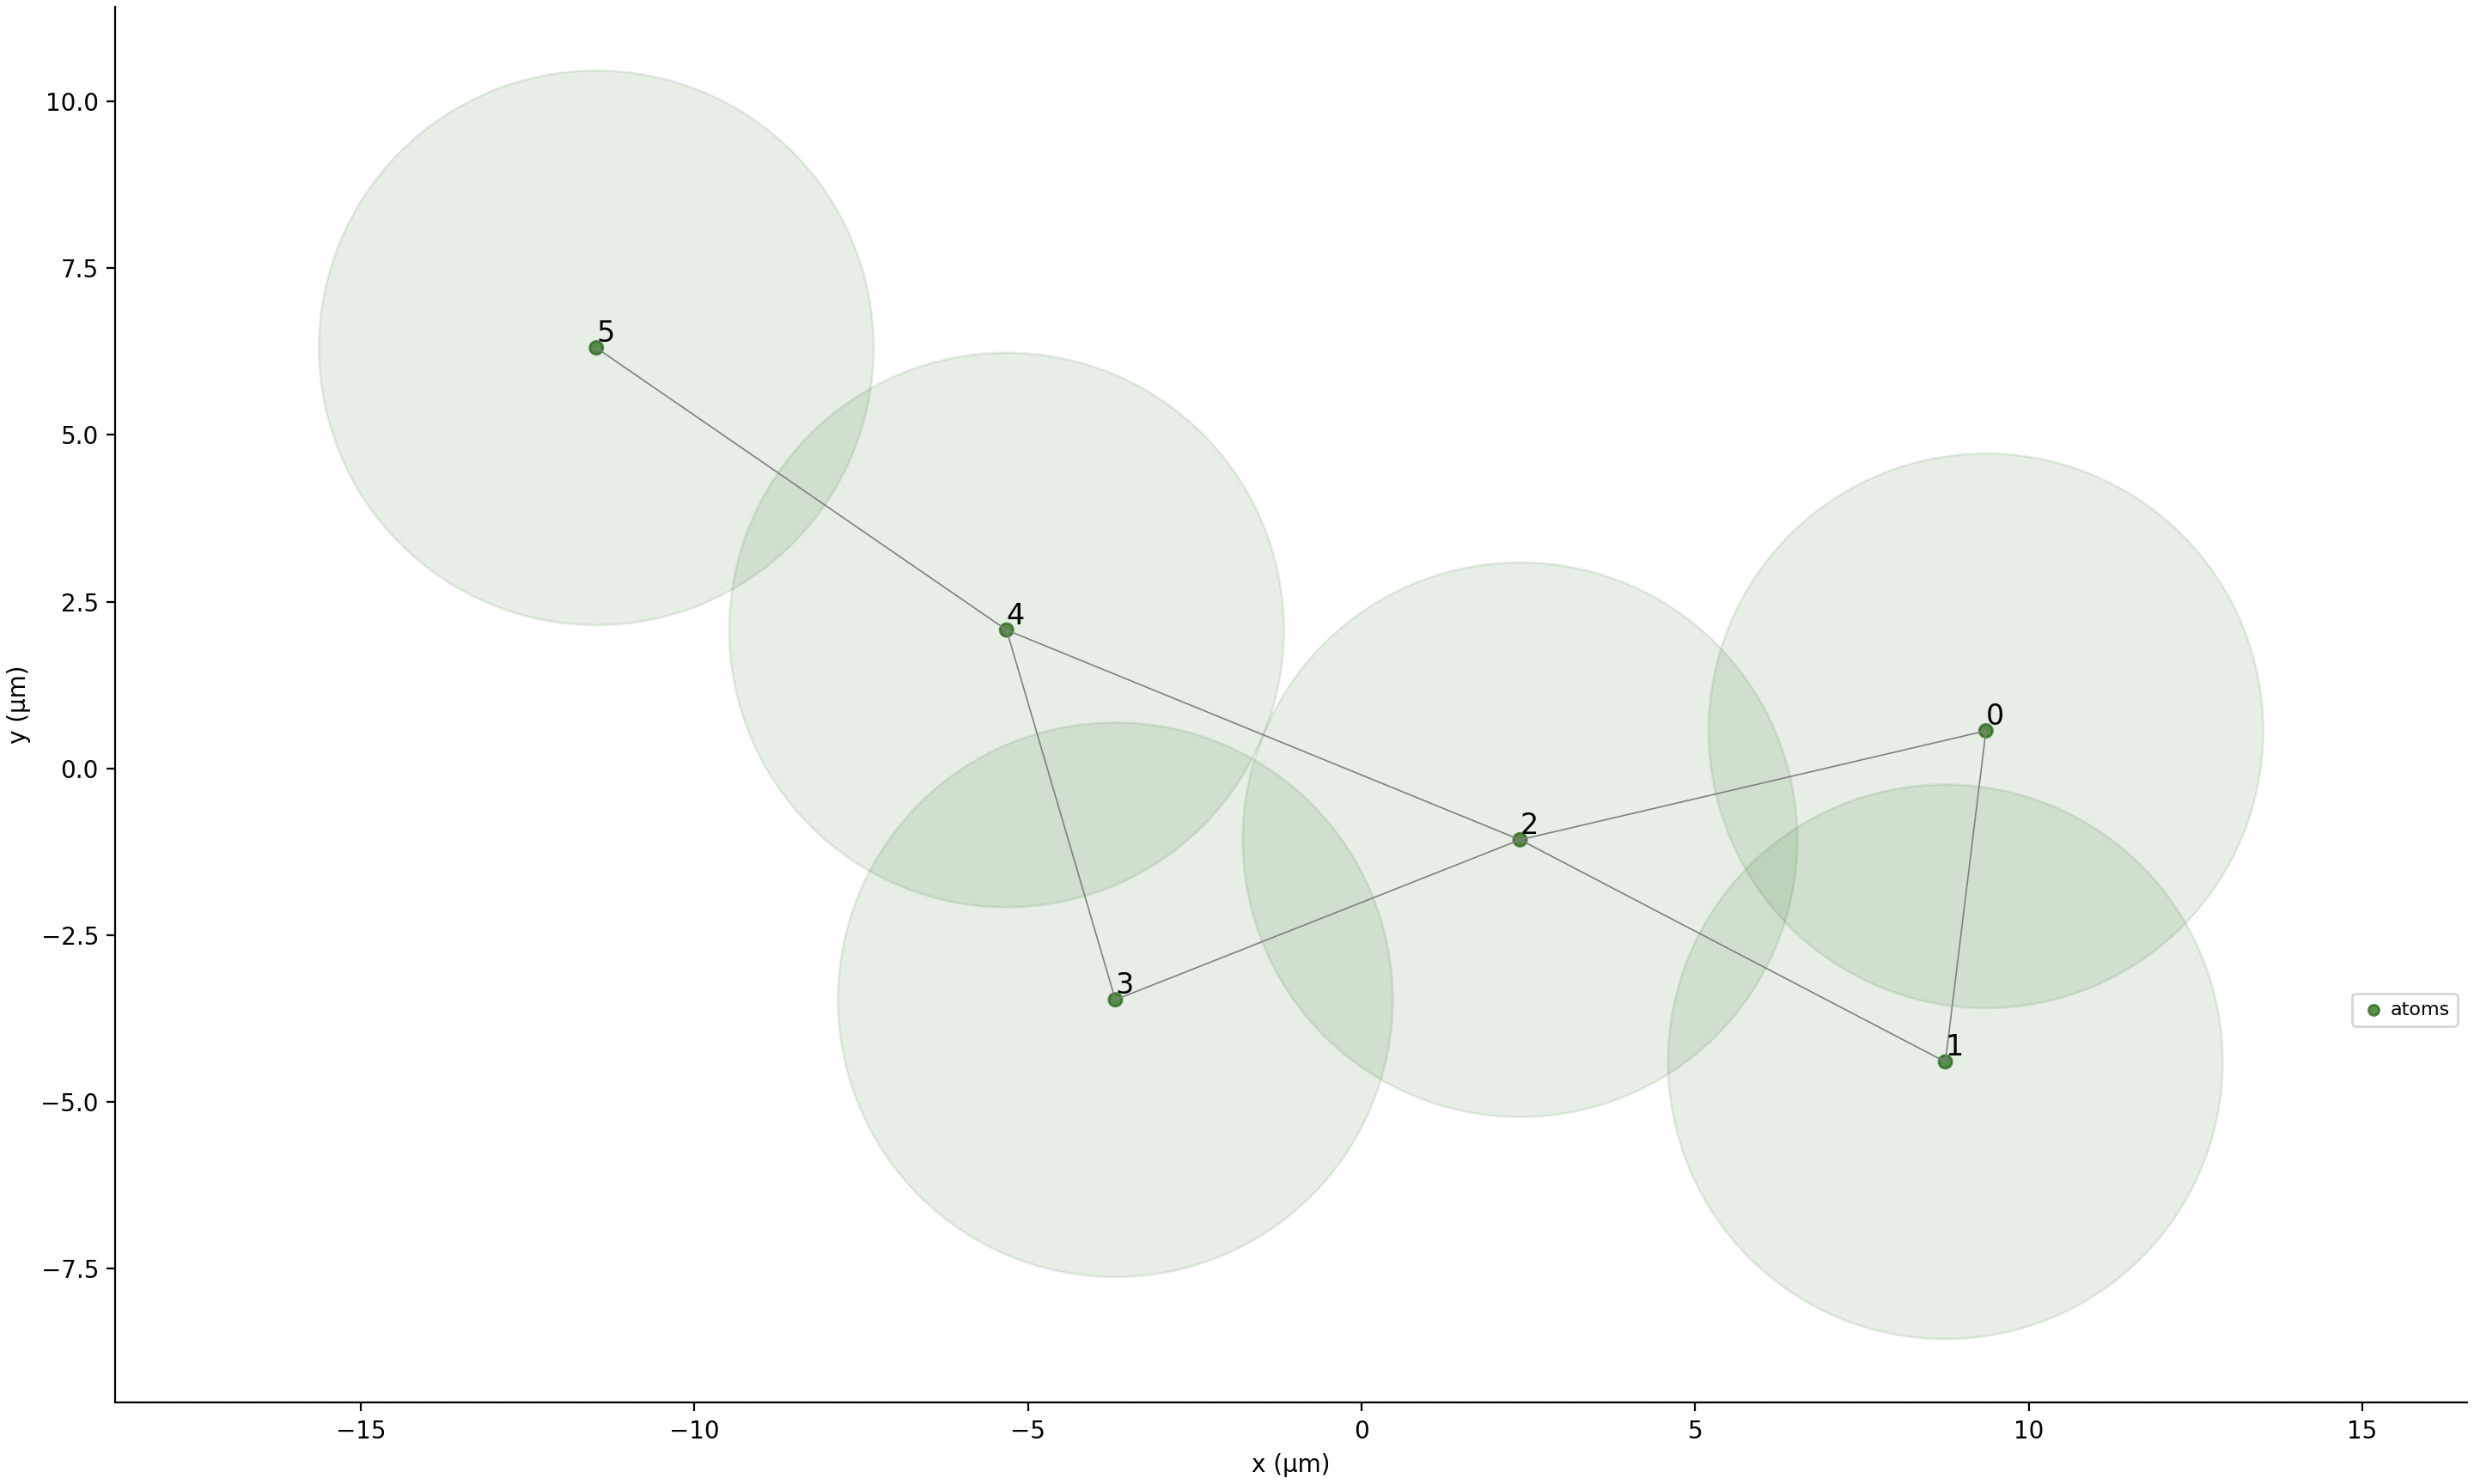
\includegraphics[width = 0.48\linewidth]{images/registre_exemple.png}
    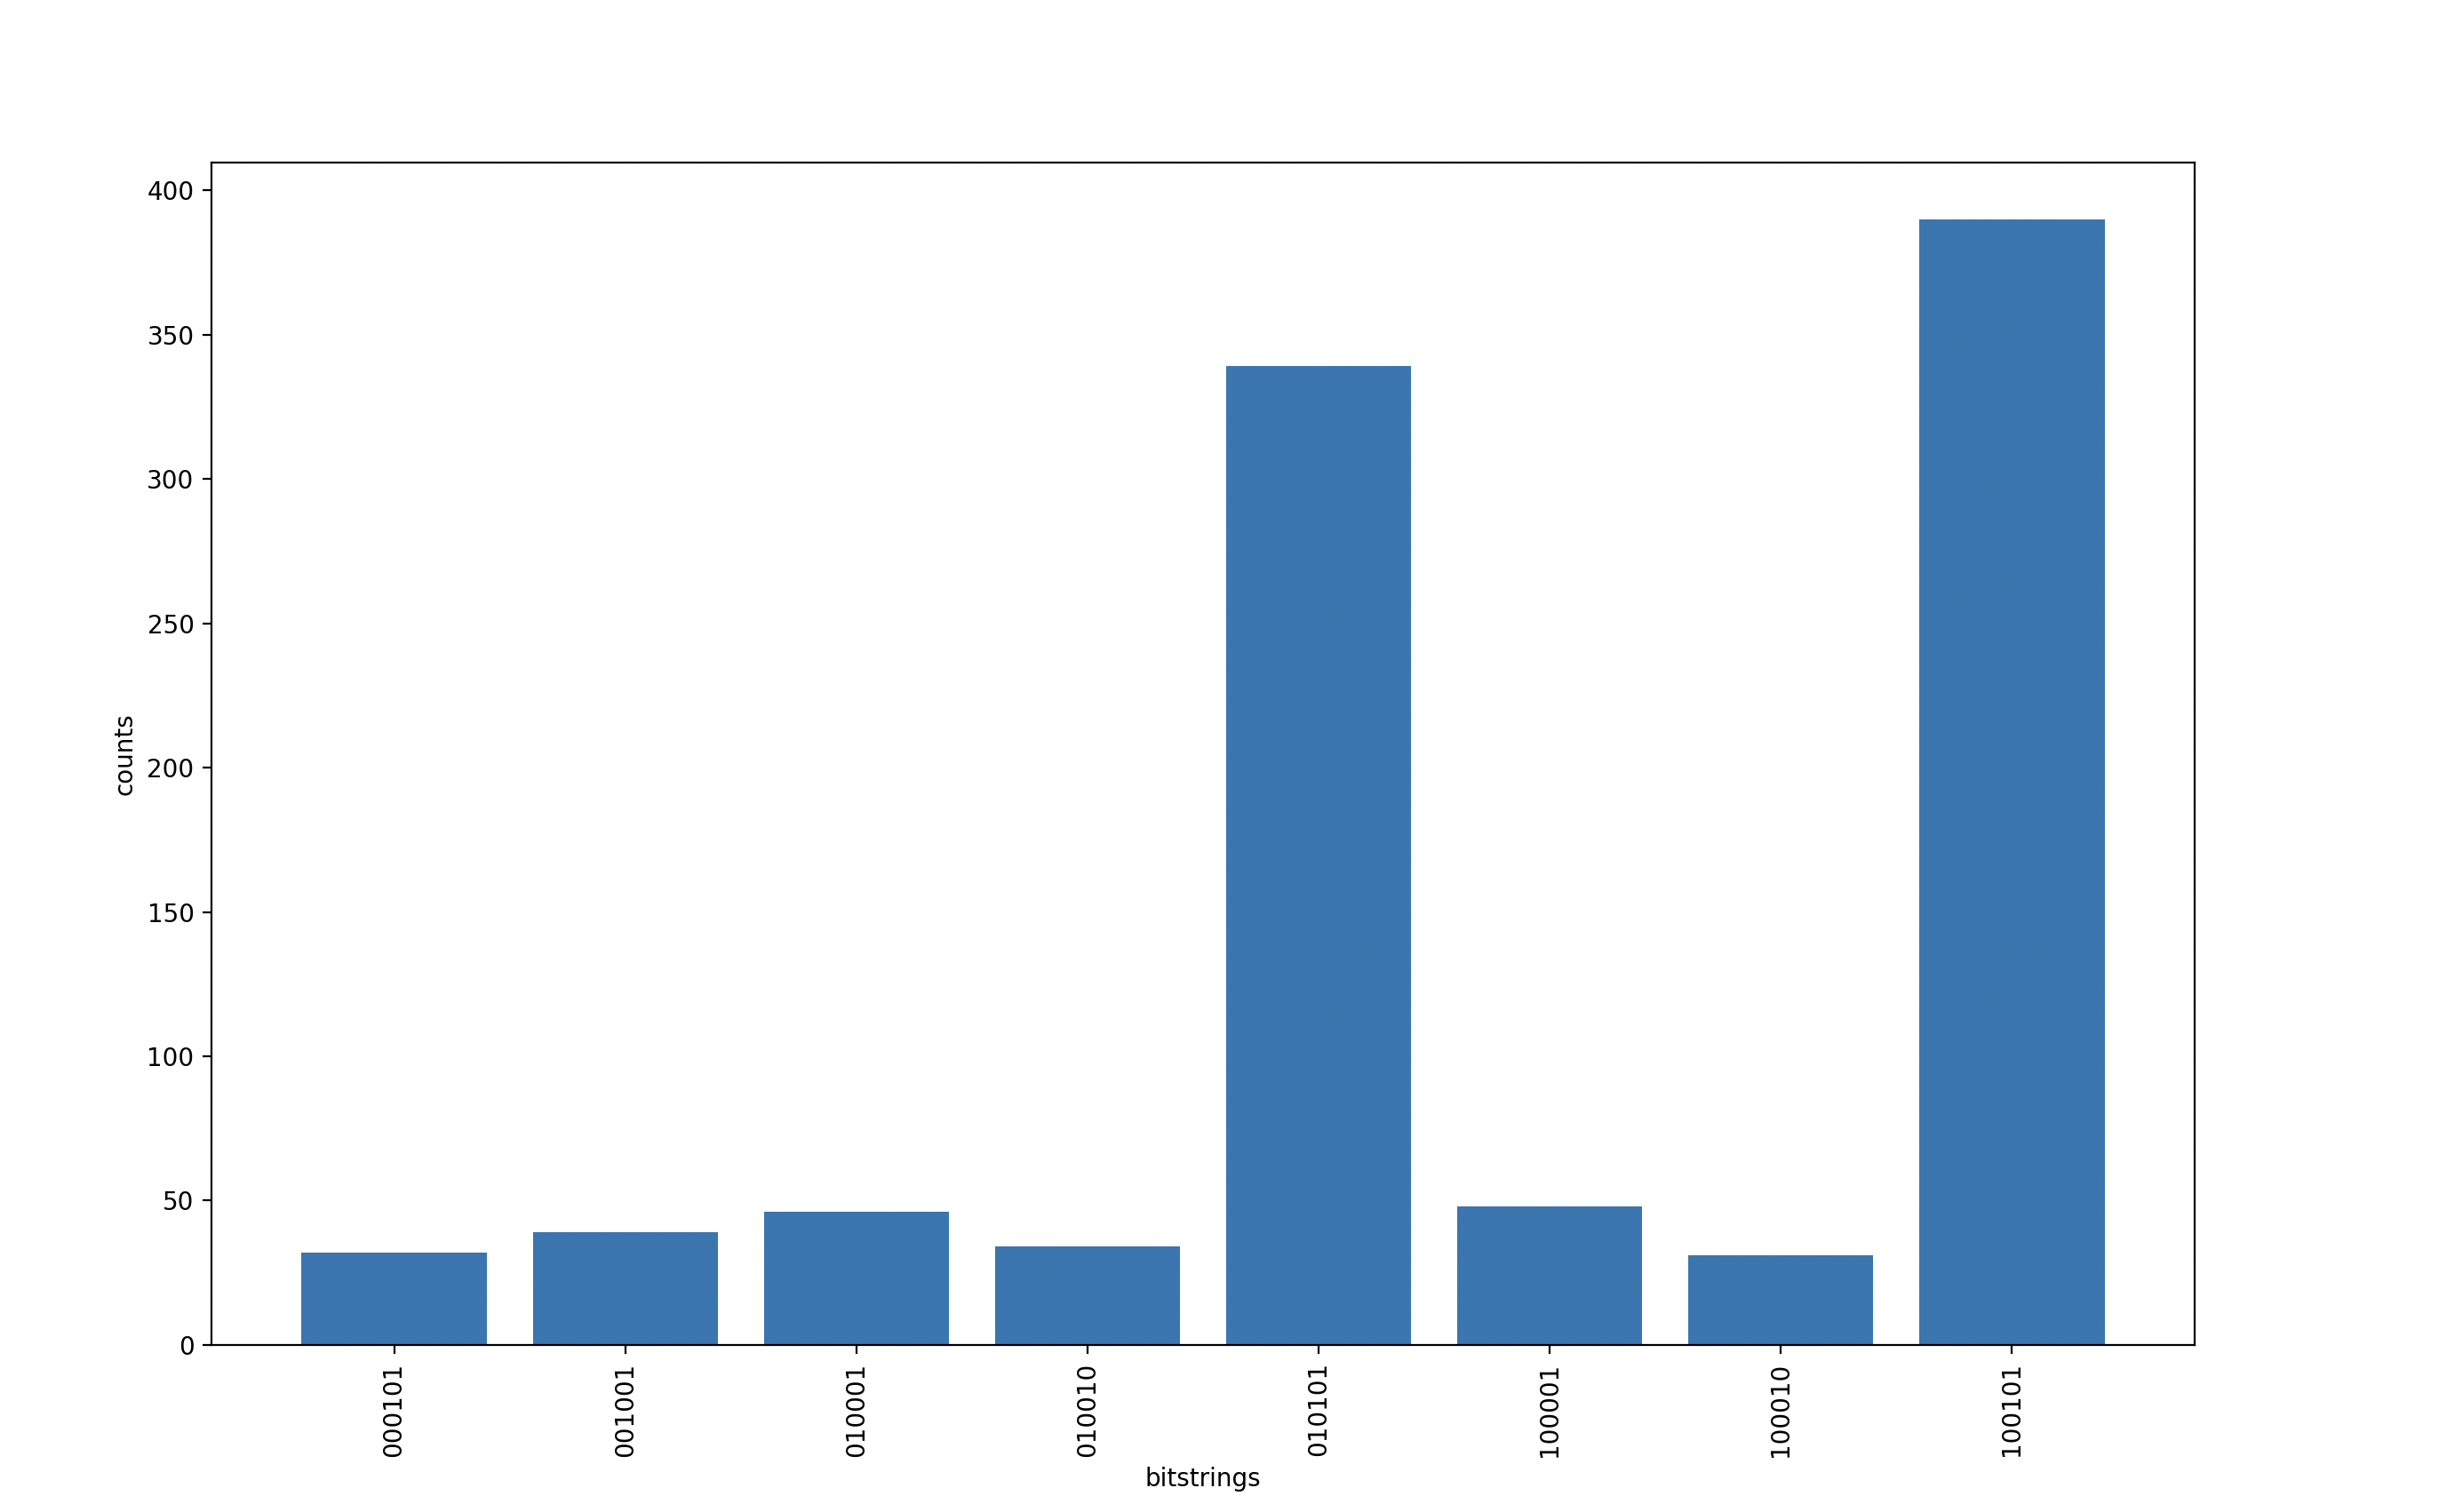
\includegraphics[width=0.49\linewidth]{images/histogram_exemple.png}
    \caption{Registre quantique et l'histogramme associé à ce registre après 1000 tentatives}
    \label{QMIS_exemple}
\end{figure}
    
On trouve donc les deux solutions: \{0, 3, 5\}, \{1, 3, 5\} qui correspondent bien aux deux solutions admises de ce graphe à la figure 2.


%Dans le cadre de notre projet avec Récupex, nous avons utilisé une approche d'un ordinateur à atomes neutres pour résoudre un problème d'optimisation combinatoire, qui est de trouver le maximum independant set (MIS) dans notre graphe. Les ordinateurs à atomes neutres, tels que ceux développés par Pasqal, manipulent des qubits representées par des atomes de Rydberg, dont l'intrication repose sur le phénomène de blocage de Rydberg. Cette méthode permet de modeliser les graphes ou les qubits interagissent en fonction de leurs emplacements dans l'espace et des pulses appliqués.
%D'autre part le problème du MIS nous permet de sélectionner les emplacements qui maximisent l'efficacité de collecte tout en minimisant les conflits potentiels dans l'emplacement des bacs (comme la proximité excessive). En utilisant une approche de calcul analogue, nous pouvons tirer parti des propriétes physiques du système quantique pour explorer rapidement et efficacement les résultats possibles, ce qui nous aidera a trouver les configurations optimales répondant aux critères et objectifs de performance de Récupex 

\subsubsection{Algorithme d'optimisation approximative quantique} 
 
 L'algorithme d'optimisation approximative quantique (\textit{QAOA}) est une méthode largement utilisée pour résoudre des problèmes d'optimisation combinatoire tels que le problème de l'ensemble indépendant maximal \cite{farhi_quantum_2014}. Le QAOA utilise des circuits quantiques pour approximer les solutions optimales des problèmes. Il repose sur la définition de deux hamiltoniens : l'hamiltonien de coût (H\_c), dont l'état fondamental encode la solution du problème d’optimisation, et l'hamiltonien de mélange (H\_m) , conçu pour explorer l'espace des états quantiques. 
 L'algorithme alterne ensuite l'application de ces deux hamiltoniens sur un état initial. À chaque étape, l'hamiltonien de coût est appliqué pendant un temps $\alpha$, et l'hamiltonien de mélange pendant un temps $\beta$.  Ces paramètres $\alpha$ et $\beta$ sont ensuite optimisés à l'aide de méthodes d'optimisation classique pour maximiser la probabilité de mesurer une solution optimale.
 Avec un nombre élevé d'étapes ( représentées par la profondeur p ), le QAOA peut théoriquement s'approcher de plus en plus de la solution optimale. Il s'impose donc comme une technique prometteuse pour aborder des problèmes complexes, notamment ceux liés aux graphes, ainsi que des problèmes industriels et logistiques.


\subsection{Ensemble maximal indépendant en sous-graphe}
Sachant que le simulateur quantique ne peut traiter que des problèmes à 25 atomes (équivalent à un graphe d'au plus 25 sommet que l'on tente de trouver l'ensemble indépendant maximal), le graphe contenant beaucoup plus de point doit être traité en sous-intences de graphe. Pour ce faire, l'algorithme METIS développé entre autre par George Karypis et Vipin Kumar est utilisé \cite{karypis_multilevelk-way_1998}. Il permet de séparer un graphe en n sous-graphes contenant environ le même nombre de sommets tout en minimisant le nombre d'arrêtes perdus dans la somme des sous-graphes. Cet algorithme sera utile puisqu'il permet de créer juste le nombre d'instances de sous-graphe nécessaire pour faire le moins de calcul quantique possible tout en gardant le plus d'information possible. 

Par la suite, pour recombiner les ensembles indépendants maximals des sous-graphes, nous allons effectuer un algorithme permettant de fusionner une paire de ceux-ci. Selon Michael Blondin, professeur en algorithmie à l'Université de Sherbrooke, il est possible de créer un ensemble indépendant maximal rapidement en prenant simplement les noeuds impliqué dans les MIS et la connexion entre les graphes. Autrement dit, en créant le graphe reliant les points du MIS des sous-graphes A et B selon les arrêtes du graphe initial. Nous n'incluons pas les sommets qui n'ont pas d'arrêtes reliant un sommet de l'autre sous-graphe.

Le graphe obtenu est acyclique et nommé forêt. Il est possible de trouver l'ensemble maximal indépendant de ce type de graphe par un algorithme classique inspiré de la programmation dynamique. Même s'il n'existe pas de garanti que la solution ne sera pas un ensemble indépendant maximal, il restera tout de même indépendant et cette recombinaison permet d'utiliser le simulateur quantique avec une bonne approximation de la réponse.

\section{Méthodologie}

\subsection{Comparer les méthodes trouvant le MIS}
\subsubsection{Choisir la méthode quantique la plus prometteuse}
L'algorithme adiabatique et d'optimisation approximative seront testés sur le graphe suivant: 

\begin{figure}[H]
    \centering
    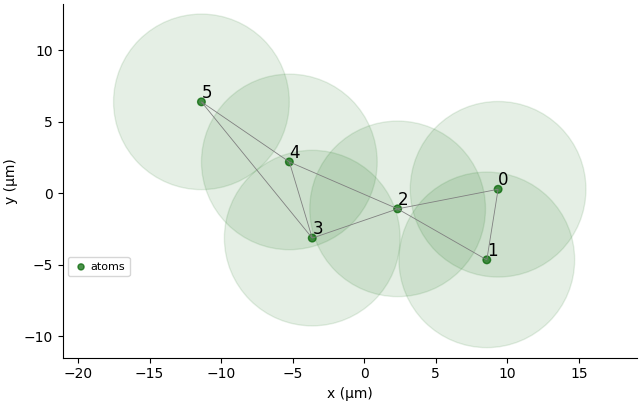
\includegraphics[width = 0.48\linewidth]{images/registre_exemple2.png}
    \caption{Graphe pour lqeul les deux algorithmes quantiques seront testés sur un simulateur}
\end{figure}\label{graphtocompare}

Les performances des algorithmes seront comparer pour déterminer la méthode à employer pour résoudre des plus gros porblèmes. En effet, les ressources pour tester les algoirthmes sont limitées. Ainsi, une seule méthode se doit d'être exploré en détail pour avoir des résultats interessants.

\subsubsection{Évaluer la performance de l'algorithme de recombinaison de sous-graphe}
Ensuite, la performance de l'algorithme de recombinaison de graphe sera testé sur un graphes de 35 sommets. Avec l'aide du puissant simulateur de Pascal permettant de rouler des algorithmes de calculs analogiques quantique à environ 35 atomes, il sera possible d'appler directement l'algorithme quantique ayant le mieux performé à l'étape précédente une seule fois pour le graphe. Ainsi, en exécutant l'algorithme classique n'ayant pas de limitations, l'algorithme quntique, nous allons pouvoir comparer la performance de ces algorithmes. Il sera aussi possible de voir si la recombinaison de sous-graphe donne une bonne approximation d'avoir rouler le graphe au complet dans un seul appel de MIS.

\subsection{Résoudre le problème de Récupex}
La réatribution des bacs plus efficace dans la ville se sépare dans les 3 grandes sections suivantes.

\subsubsection{Tri de l'emplacement actuel des bacs}
La première étape consiste à retirer des bacs dans leur répartition actuele. En effet, en utilisant l'algorithme du stable maximum (MIS), des bacs seront enlevés. Le graphe sera construit comme suit:
\begin{itemize}
    \item Les bacs représenteront les sommets su graphes.
    \item Deux sommets du graphe sont reliés si les bacs en question sont à 1,5 km ou moins de distance. Par contre, cette arrête est retiré si le volume moyen annuel de vêtement reçu de chacun des bacs impliqué est de plus de 27754 (ce nombre est la somme de la moyenne des volume et l'écart-type). Les données de volumes récoltés annuels sont directement fournis par Récupex.
\end{itemize}
Des solutions données, nous prenons celle maximisant le volume de don total. Notons $n$ le nombre de bacs retirés par le MIS.

\subsubsection{Rafiner la liste des endroits possibles}
Avec les données de l'esemble indépendant maximal résultant, les commerces à un rayon de 1,5 km d'un bac seront retiré de la base de données des emplacements possibles de bacs. Les emplacements possibles sont discutés dans la théorie.

\subsubsection{Trouver les nouveaux endroits des bacs retirés}
Par la suite, un graphe sera créé avec la liste rafinée des endroits possibles pour mettre les bacs.
\begin{itemize}
    \item Les sommets seront les endroits possibles.
    \item Deux sommets seront reliés par une arrêtes si la distance entre leur endroit possible associé est moins de 2,8 km. Par la suite, un algorithme de MIS sera utilisé pour obtenir la nouvelle distribution des bacs.
\end{itemize}

Le choix des distances est arbitraire. Le choix a été fait dans le but d'obtenir une nouvelle distribution d'environ 60 bacs.
Cette méthodologie sera exécutée pour la méthode classique où chacun des MIS sera exécuté 100 fois pour obtenir le résultat apropriée selon l'étape (décrit plus haut).
Elle sera aussi exécuté avec la méthode trouvant des MIS en divisant en sous-graphes où chacun des sous-smis est exécuté 100 fois avec le pulse  "Rise-Fall" de $4000 \mu s$ avec la méthode quantique adiabatique. La première étape sera fait avec des sous-graphe d'au plus 10 atomes et la deuxième avec au plus 7 atomes. Ces paramètres ont été choisis après plusieurs tests parcqu'ils donnaient la meilleur distribution.



\section{Résultats}
\begin{figure}[H]
    \centering
    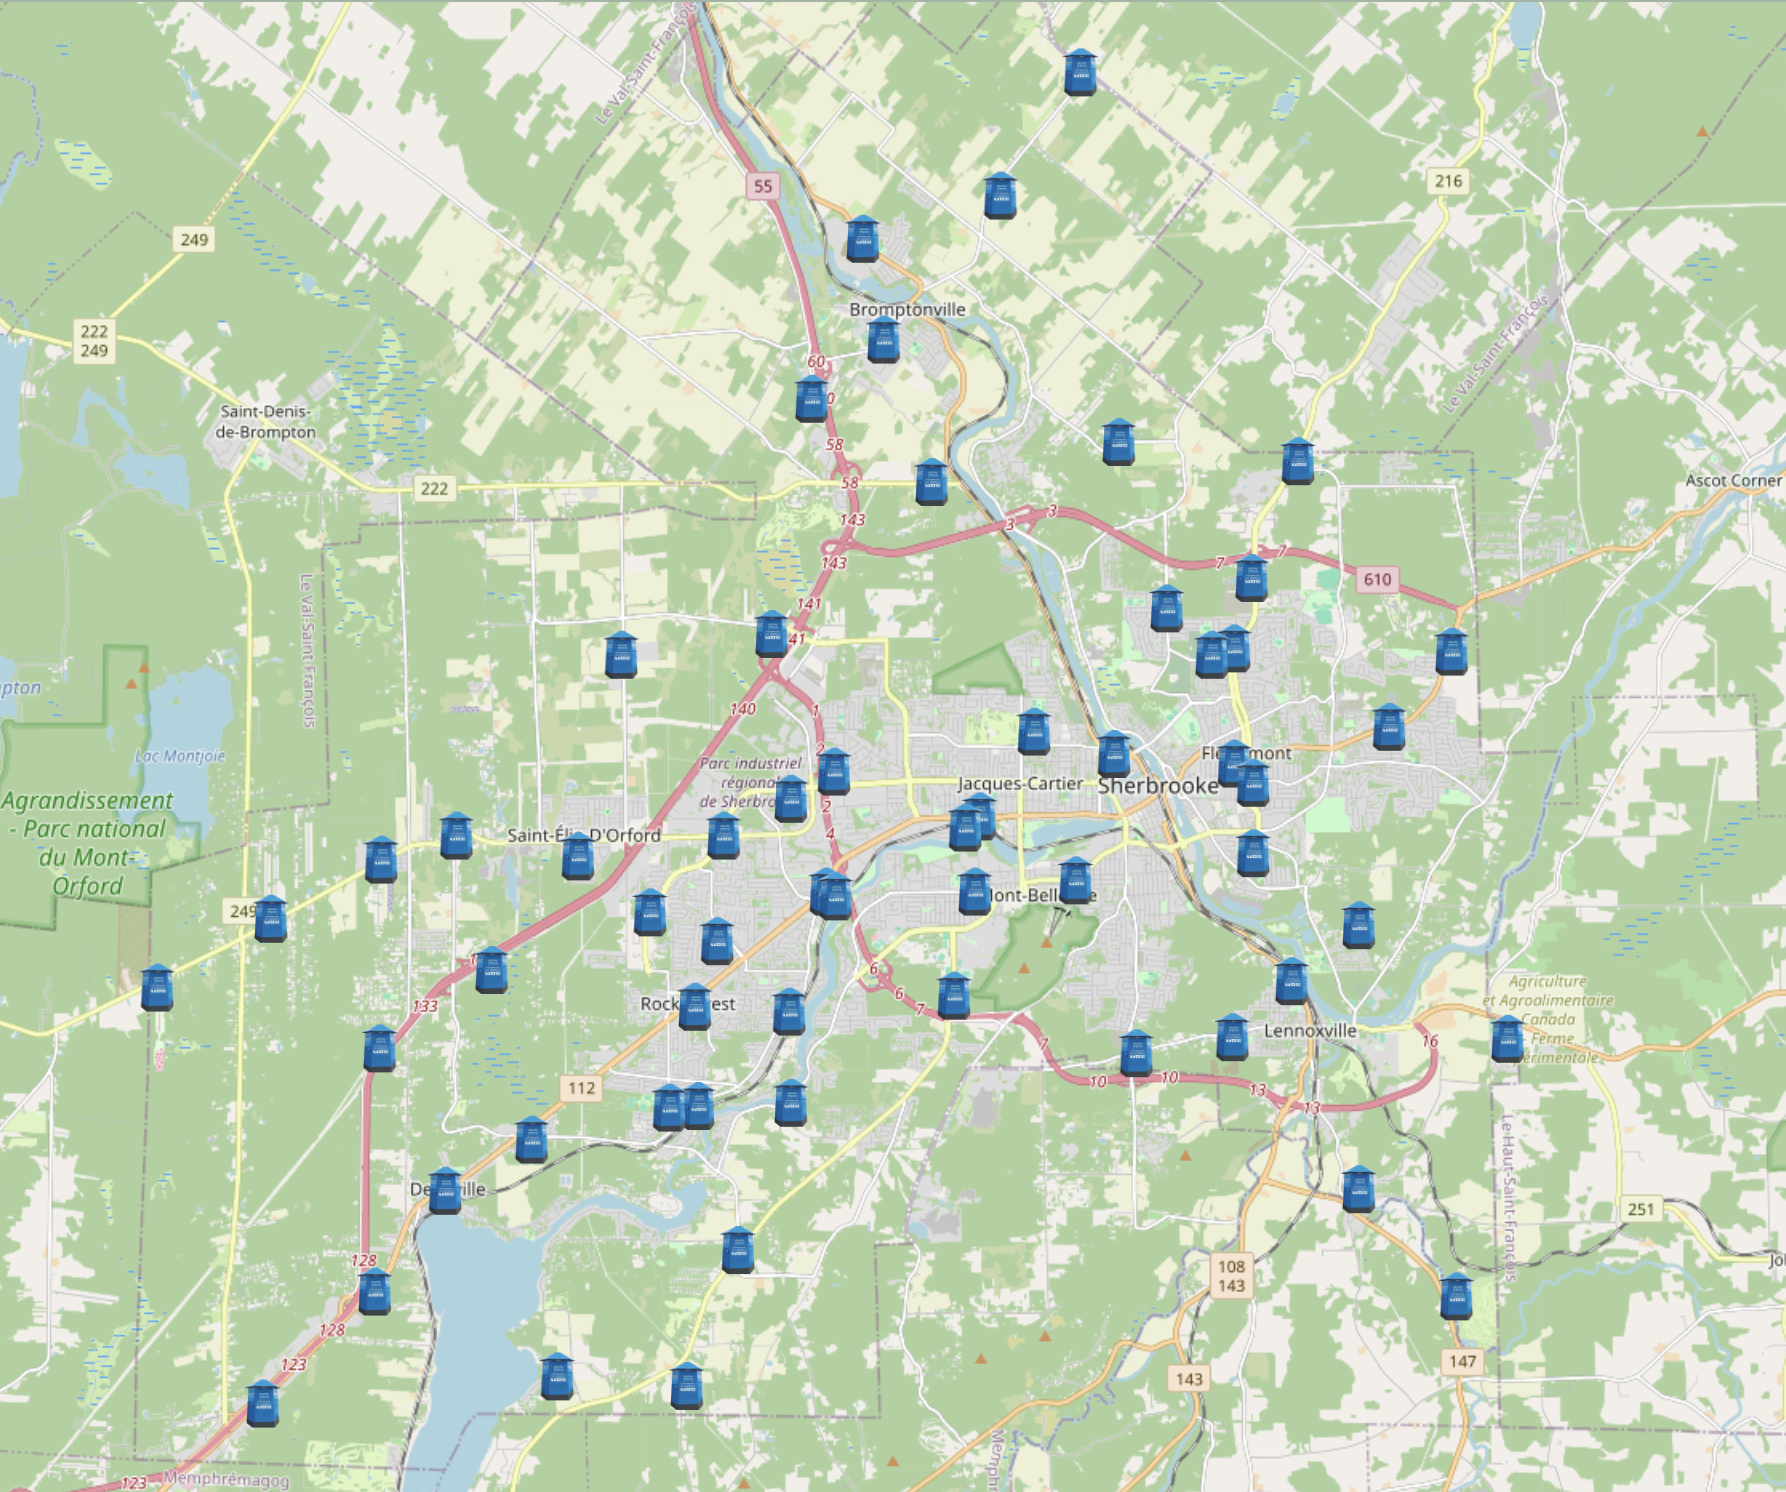
\includegraphics[width=0.49\linewidth]{images/new_quantum.png}
    \caption{Répartition des bacs après l'usage de notre algorithme quantique}
    \label{new_quantum}
\end{figure}
\begin{figure}[H]
    \centering
    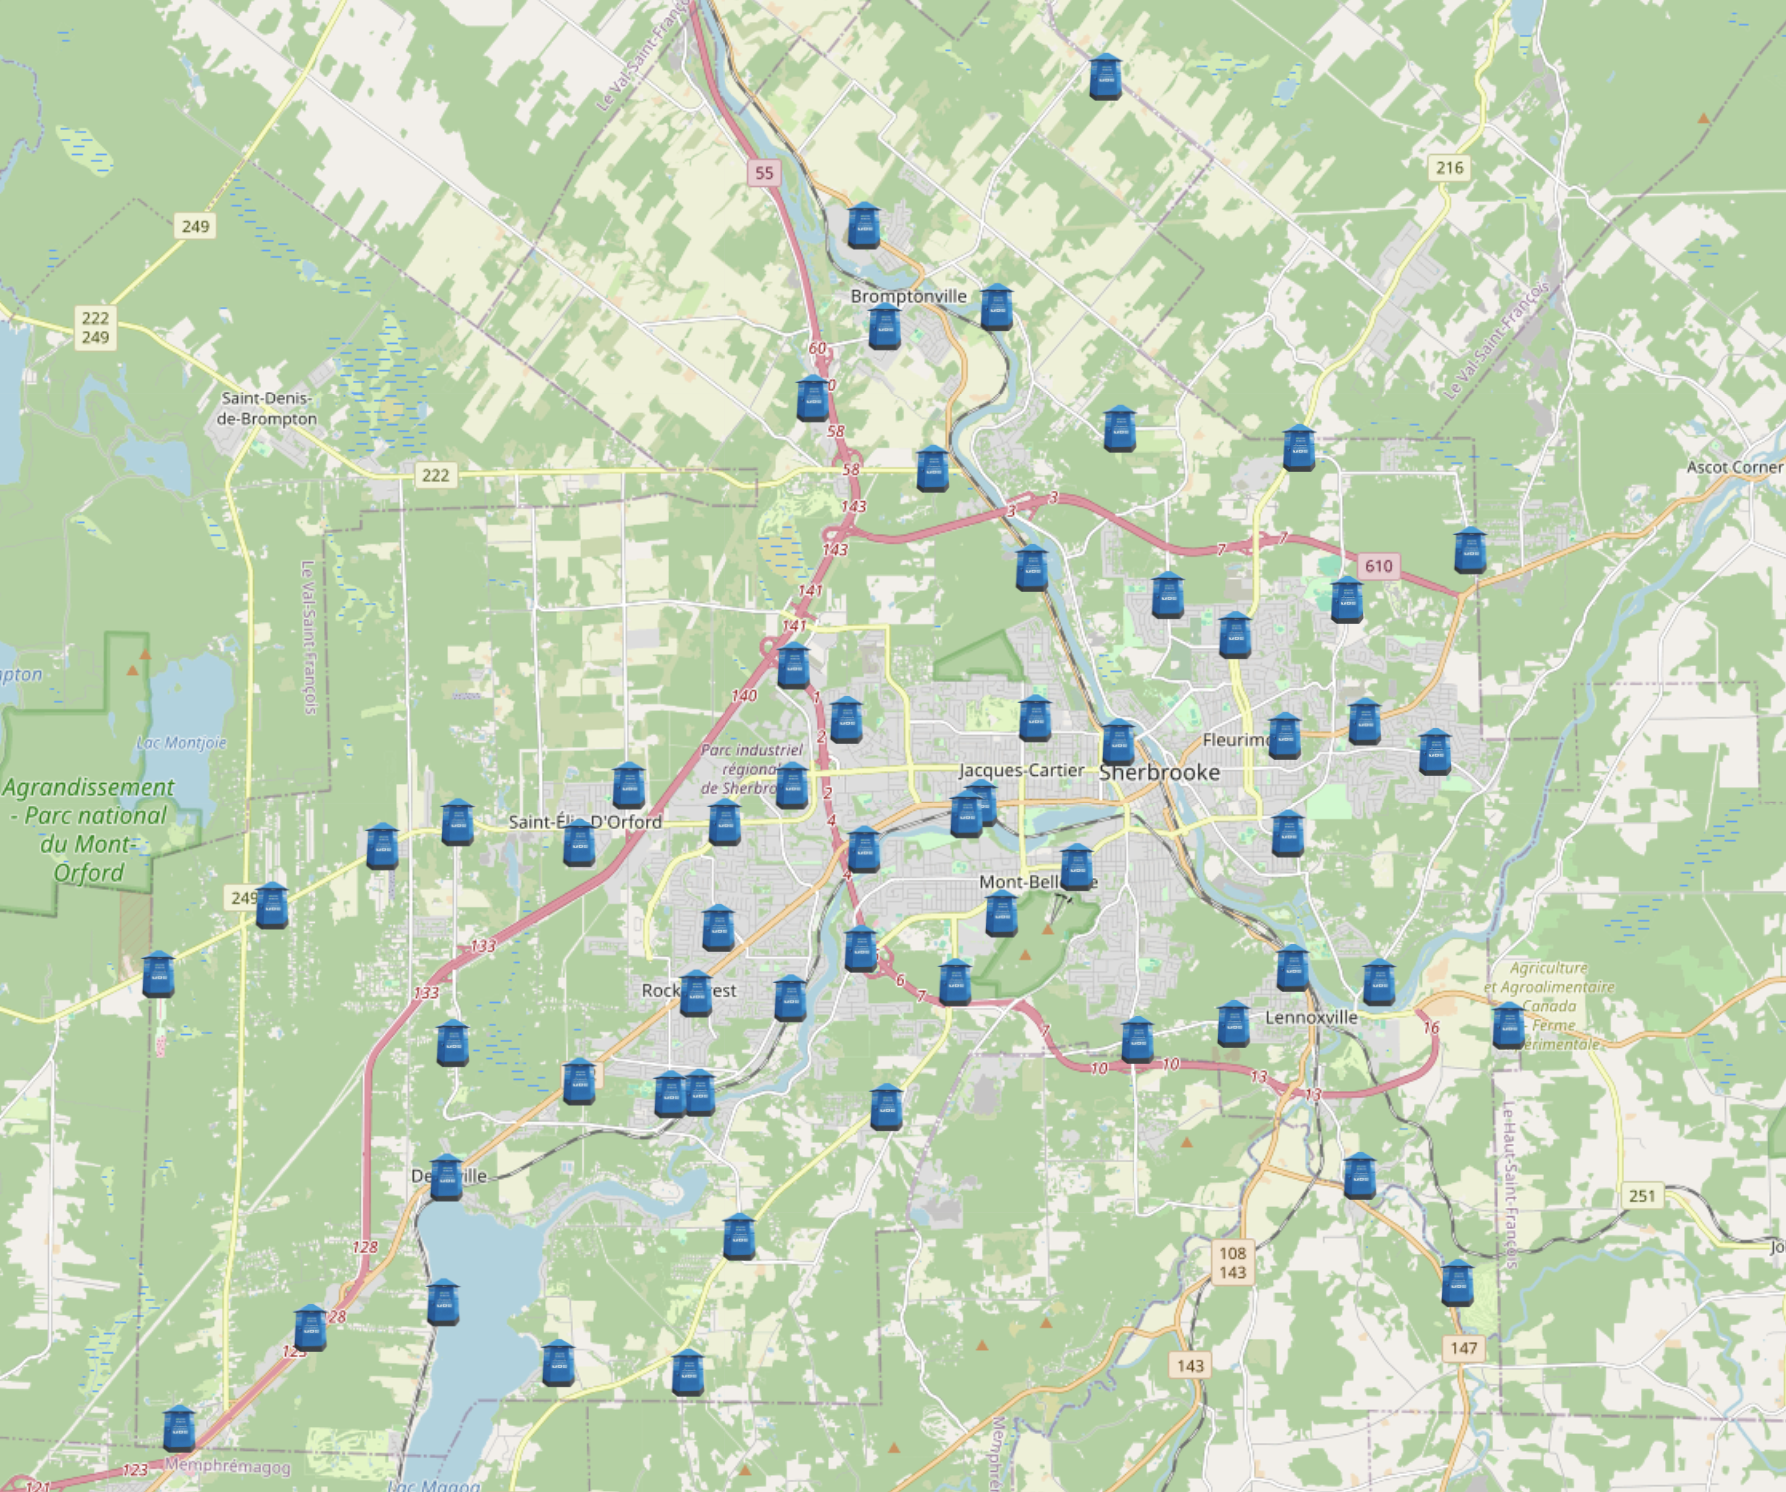
\includegraphics[width=0.49\linewidth]{images/new_classical.png}
    \caption{Répartition des bacs après l'usage de notre algorithme classique}
    \label{new_classical}
\end{figure}
\begin{figure}[H]
    \centering
    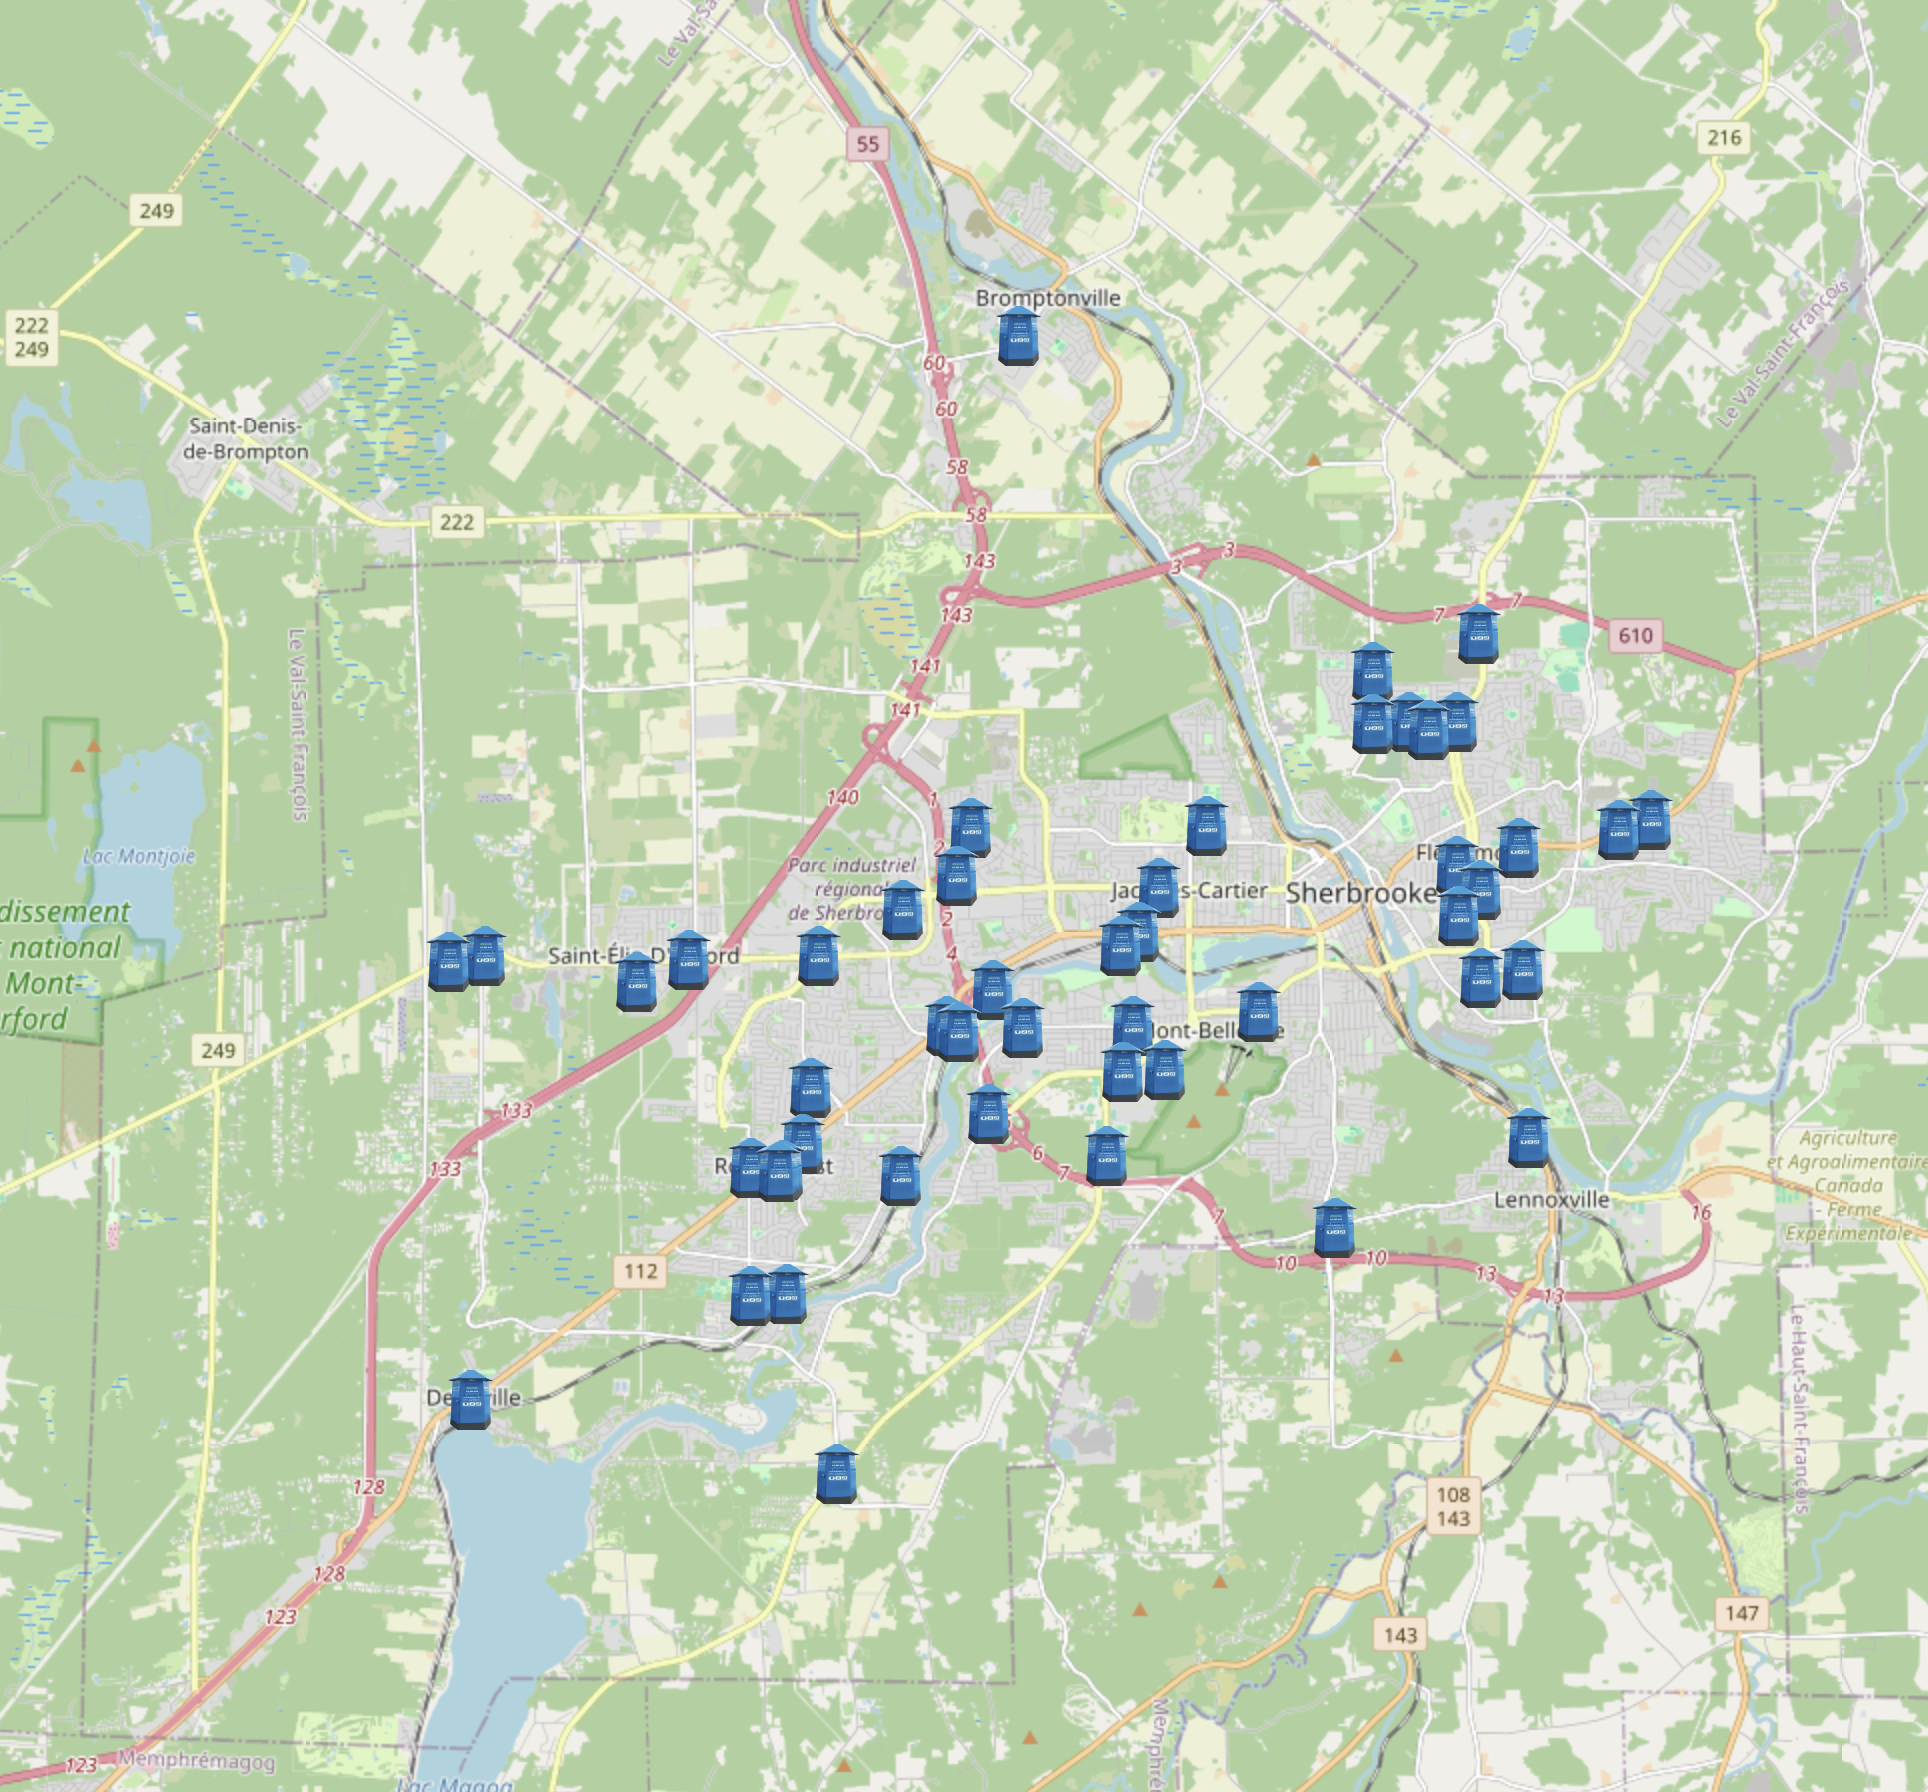
\includegraphics[width=0.49\linewidth]{images/original.png}
    \caption{Répartition des bacs à l'origine}
    \label{original}
\end{figure}
\begin{figure}[H]
    \centering
    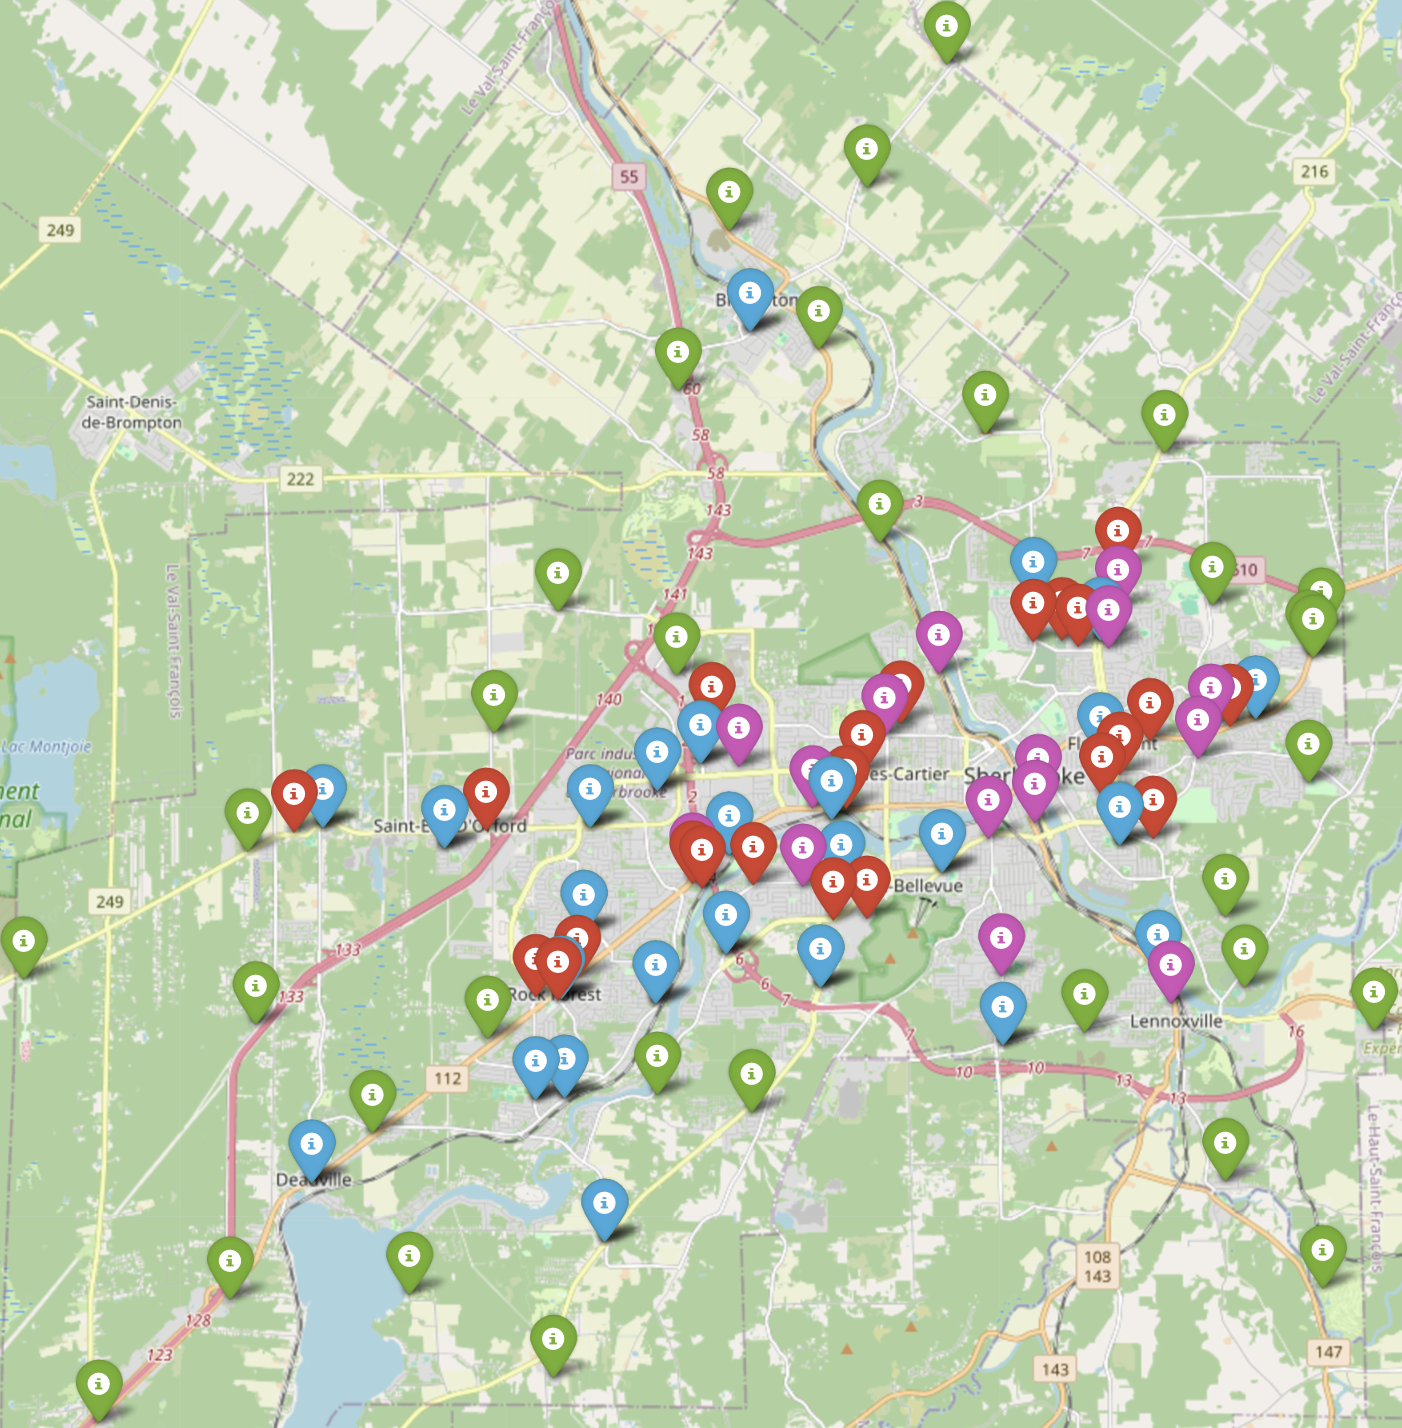
\includegraphics[width=0.49\linewidth]{images/total_quantum.png}
    \caption{Carte des cloches après l'usage de notre algorithme quantique (les points \textcolor{Mulberry}{violets} représentent les bacs d'Estrie-Aide, les points \textcolor{LimeGreen}{verts} représentent les bacs ajoutés, les points \textcolor{BrickRed}{rouges} représentent les bacs enlevés les points \textcolor{CornflowerBlue}{bleus} représentent les bacs conservés).
}
    \label{total}
\end{figure}

\begin{figure}[H]
    \centering
    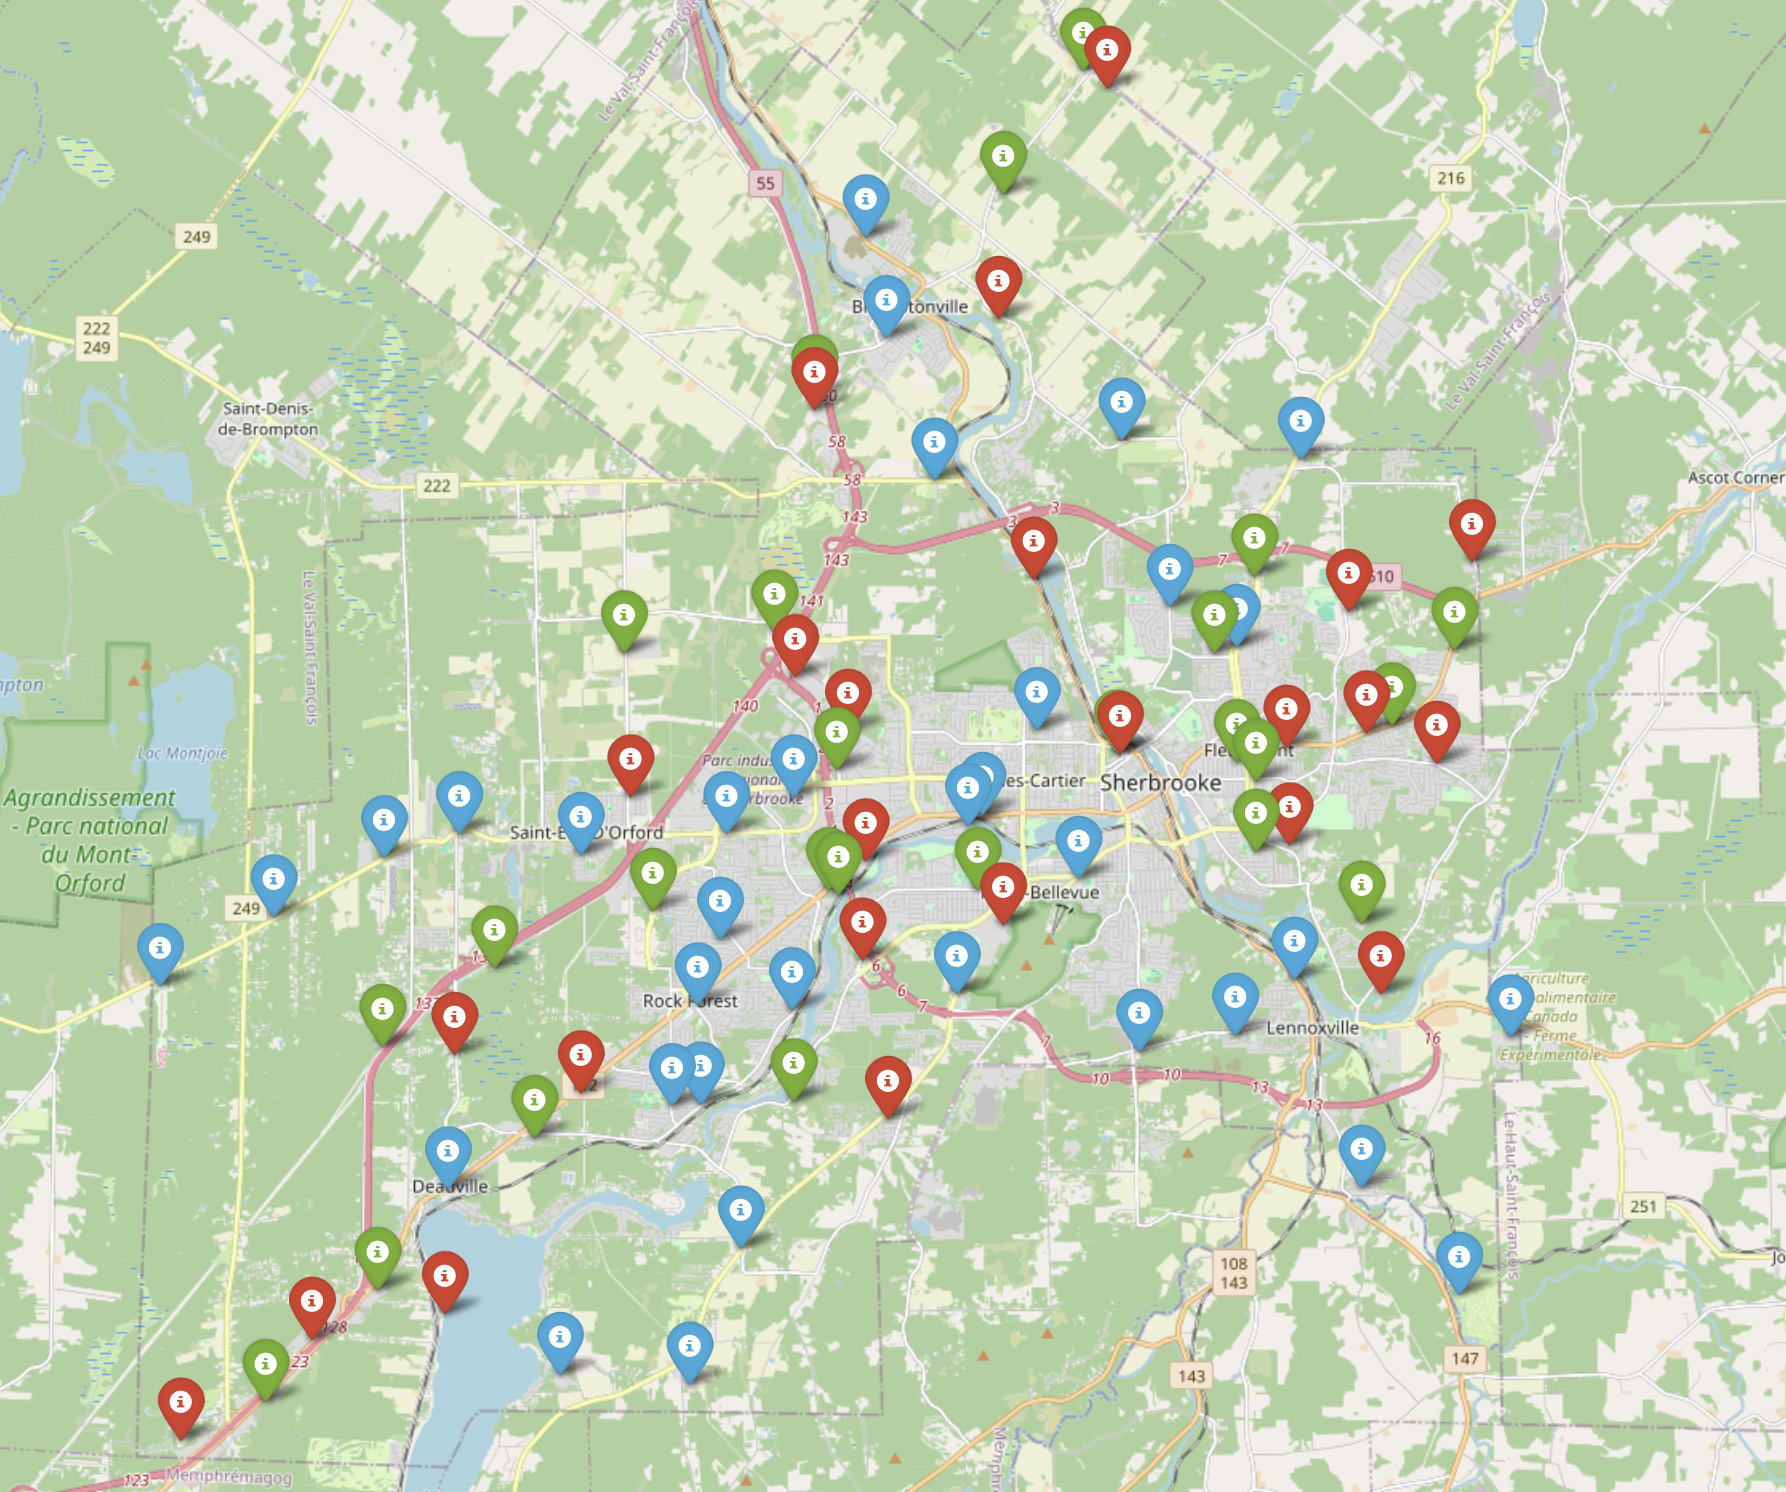
\includegraphics[width=0.49\linewidth]{images/both_distributions.png}
    \caption{Carte de la compariaosn des emplacements choisis par la méthode classique et quantique (les points \textcolor{LimeGreen}{verts} représentent les bacs seulement dans la distribution des bacs obtenus par la méthode quantique, les points \textcolor{BrickRed}{rouges} représentent les bacs seulement dans la distribution des bacs obtenus par la méthode classique et les points \textcolor{CornflowerBlue}{bleus} représentent les bacs observés dans les deux distributions).
}
    \label{bothdist}
\end{figure}

\section{Discussion}
Pertinence de notre solution obtenue...

\subsection{Algorithme d'optimisation approximative quantique}
En plus de l'algorithme quantique adiabatique (\textit{Quantum Adiabatic Algorithm}) , nous avons également évalué l'efficacité de l'algorithme d'optimisation approximative quantique (\textit{Quantum Approximate Optimization Algorithm}) avec un problème MIS (\textit{Ensemble Independant Maximal}) dans ce projet. 
[[ On a commencé par la création d'un registre où les interactions entre les qubits sont déterminées par les positions des nœuds du graphe et le rayon de blocage. Ce rayon correspond à la distance minimale entre deux qubits pour éviter les interactions non souhaitées. ( deja explique dans la paragraphe precedente .. est ce que je dois le refaire .. ?) ]] 
 
L'algorithme QAOA alterne entre deux pulses sur \( p \) couches, chacun représentant un Hamiltonien spécifique. Le premier, appelé \textit{Hamiltonien de mélange} (\textit{mixing Hamiltonian}), est paramétré par \( \Omega \) et \( T_{\text{mixer}} \) et est conçu pour permettre l'exploration de l'espace des solutions. Le second, appelé \textit{Hamiltonien de coût} (\( H_q \)), encode la fonction objectif à optimiser. Ce deuxième pulse, paramétré par \( \Omega \) et \( T_{\text{cost}} \), oriente l'évolution du système vers des états correspondant aux solutions optimales.

En appliquant cette méthode sur le graphe de la figure 1, les résultats obtenus sont présentés dans l'histogramme ci-dessous. On peut observer que les bitstrings correspondant aux solutions optimales sont présents, mais pas avec la fréquence la plus élevée. Cela s'explique par la profondeur limitée du circuit QAOA, qui empêche l'algorithme de converger pleinement vers les solutions optimales. De plus, d'autres bitstrings non optimaux apparaissent avec des fréquences significatives, ce qui reflète une exploration plus variée de l'espace des solutions.
En comparaison, les résultats obtenus avec la méthode QAA (\textit{Quantum Adiabatic Algorithm}) montrent une concentration beaucoup plus marquée sur les solutions optimales, ce qui est representée l'histogramme correspondant. Cela prouve que, bien que le QAOA permette une exploration plus large, il est moins déterministe que le QAA.


\begin{figure}[H]
    \centering
    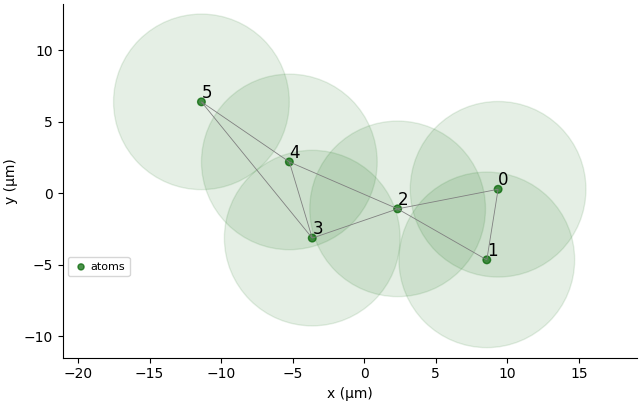
\includegraphics[width = 0.48\linewidth]{images/registre_exemple2.png}
    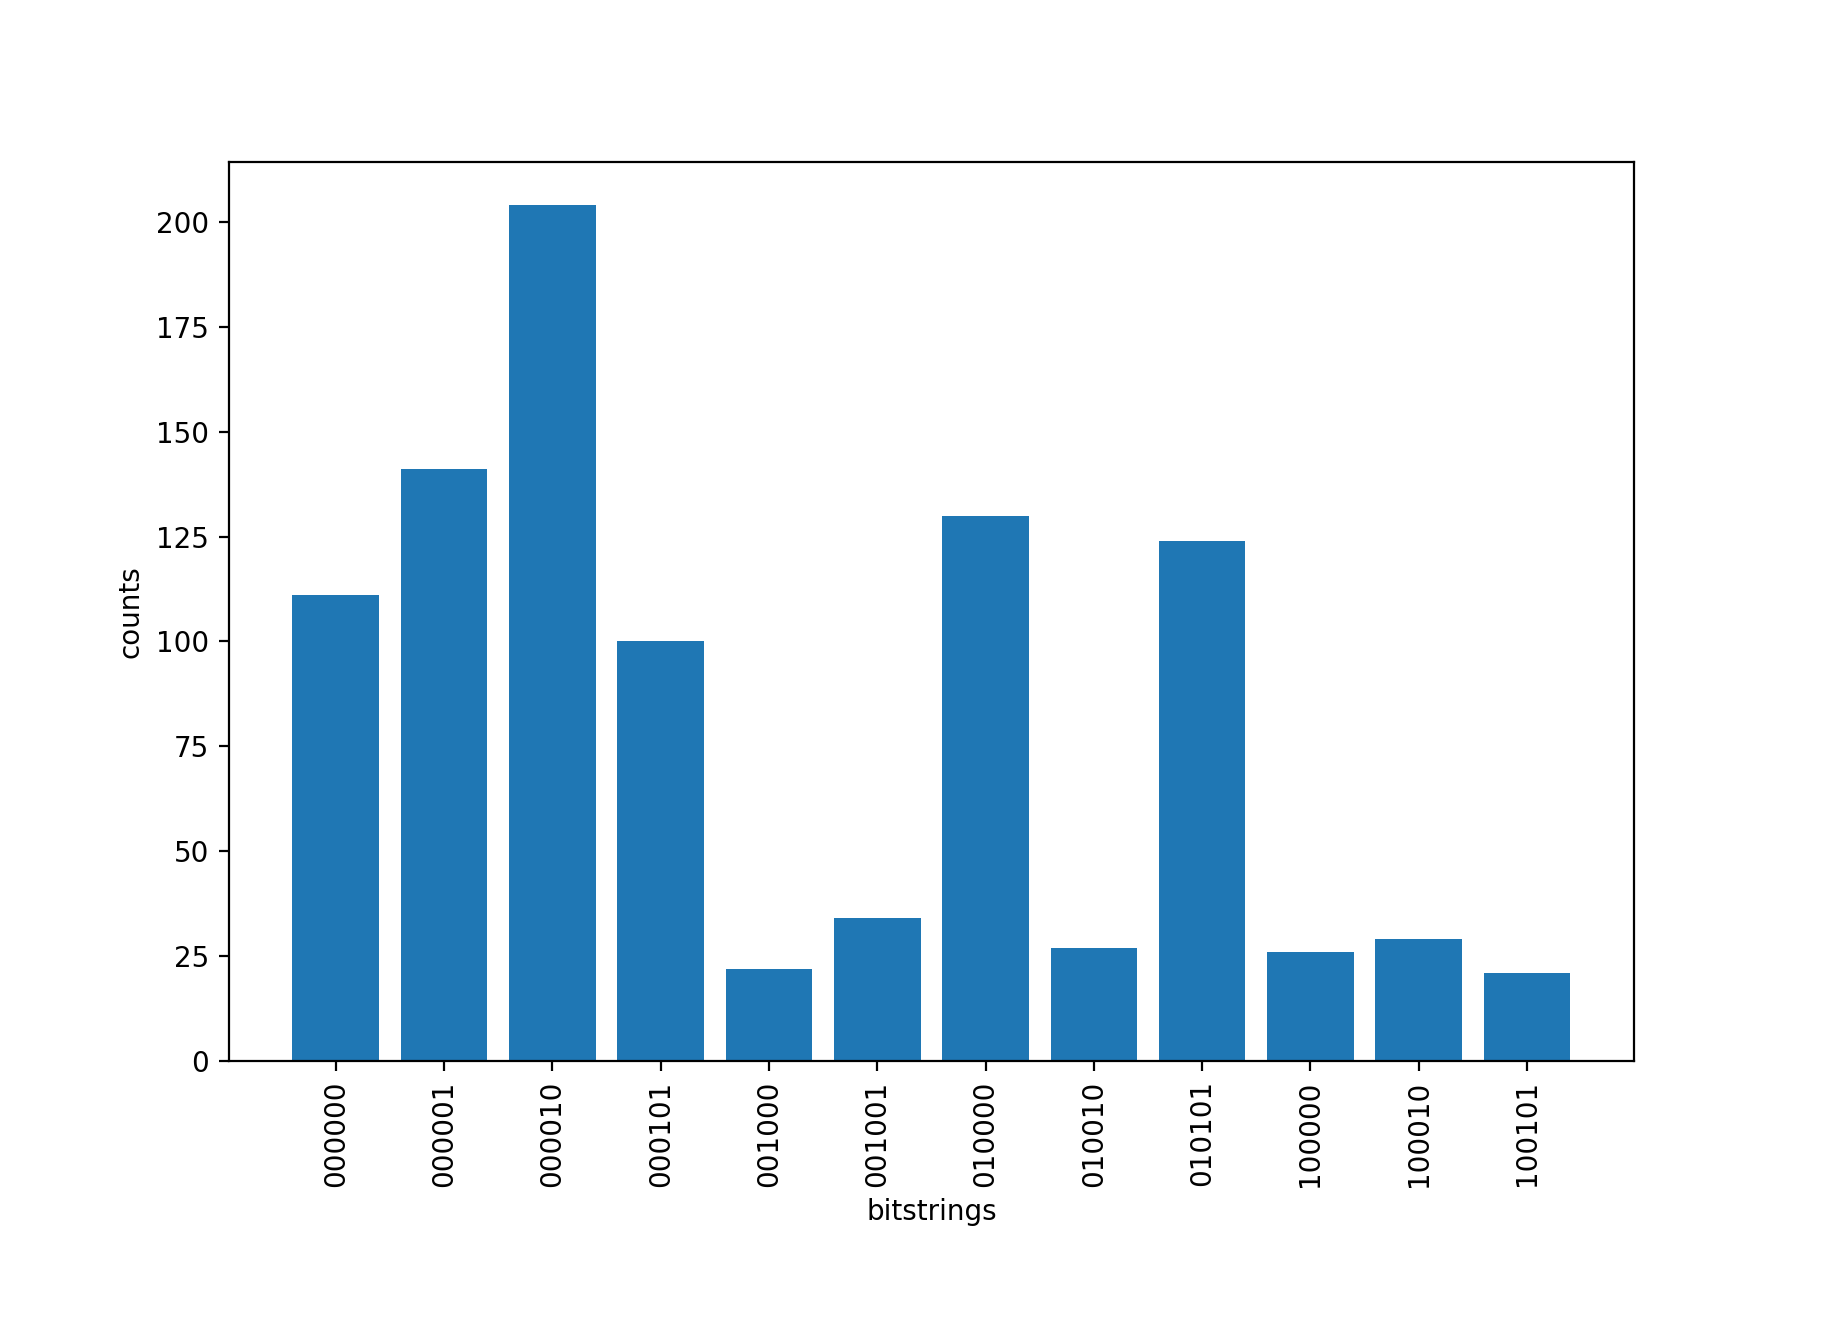
\includegraphics[width=0.49\linewidth]{images/histogram_exemple2.png}
    \caption{Registre quantique et l'histogramme associé à ce registre}
    \label{QMIS_exemple}
\end{figure}

Ainsi, bien que cette méthode soit moins limitée en termes de coût, elle nécessite une profondeur de circuit importante pour obtenir des résultats satisfaisants, ce qui rend l'optimisation plus complexe. Une conclusion similaire a été observée dans le tutoriel de Pasqal (citer ici) avec un problème QUBO (\textit{Quadratic Unconstrained Binary Optimization}).

En conclusion, bien que l'algorithme d'optimisation approximative quantique ne soit pas la méthode optimale pour un problème comme le MIS, il constitue néanmoins une approche alternative intéressante à explorer pour d'autres types de problèmes, où il pourrait offrir de meilleures performances.

\subsection{Performance de l'algorithme de recombinaison de graphe}
Comme montre la compilation des résultats de la teable \textbf{XXXX}, nous remarquons que l'algorihtme de recombinaison de graphe quantique donne un MIS près des solutions données par la méthode classique et la version quantique avec plus d'atomes. Il est évident que l'ensemble indépendant retourné n'est pas maximal. Par contre, il donne une bonne pproximation du résultat final. Il est donc pertinent de l'utiliser pour le plus grand problème de Récupex du aux graphes ayant trop de sommets pour le simulateur. Dans un monde idéal où le nombre d'atome sur l'ordinateur ne serait pas limité, la division du graphe en sous-graphe ne serait pas pertinent. En effet, un MIS serait directement calculé sur le grand graphe. Cette recombinaison de graphe permet d'utiliser l'information quantique sur un grand problème même avec ses limitations actuelles. 

De plus, la performance du simulateur est assez similaire à celle de la méthode classique. \textbf{À VOIR SI C'EST MÊME MEILLEUR....}


\subsection{Algorithme quantique adiabatique}
On en parle dans l'autre avant??

\subsection{Performance pour la résolution du problème de Recupex}
Pour résoudre le problèem de Recupex, la méthode QAA et classique on t été utilisé. En effet, comme mentionné plus tôt, la méthode de "QAOA" ne donnait pas des résultats satisfaisant sur des petits graphes. 

Il est possible de remarquer que la méthode classique donne des résultats beaucoup plus rapidmeent que le QAA. Effectivement, le fait de rouler plusieurs simulations quantiques prends beaucoup de temps. Même si sur un ordinateur quantique le temps de calcul sera moindre, le fait de préparer le système d'tome neutre 100 fois par sous-graphe prend aussi beaucoup de temps. Il y a donc un avantage d'utiliser la méthode classique lorsque plus d'emplacement possibles seront considérés. De plus, la figure \ref{bothdist} indique que les deux méthode font tout de même une bonne distriburion des bacs en choisissant une majorité de même bacs. En effet, cela indique que le premier ensemble indépendant trouvé maximisant le volume est semblable pour les deux méthodes.  Par lasuite, à l'ajout des nouveaux bacs, quelques différences sont notés par la grandeur du réseau d'emplacement possible et leur interconnection. Dans les deux cas, les deux méthodes ont réussi à bien couvrir la surface de sherbrooke en entier. Par contre, le résultat proposé par la version quantique est limité à des sous-graphes traités par la méthodes quantique à 10 sommets pour la première partie et la dernière partie à 7 sommets. En faisant cela, les MIS résultants des sous-graphes ne sont pas autant significatif que souhaité puisque la majorité des calculs se fait par la recombinaison de plusieurs petits sous-graphes ayant une réponse triviale qui ne nécisseterait pas le quantique. Des avanues pour résoudre ce roblème seront présentés dans la prochaine section.



----------------




Il faut considérer le nombre de ressources qui sont utilisées pour obtenir nos résultats. ...

\section{Pistes d'amélioration}


La création d'un registre de façon générale pour un graphe de disque unitaire limite notre algorithme quantique puisque le registre est mal généré pour des graphes non-connexes. Nous devons utiliser moins d'atomes et nous perdons donc en précision lors de l'étape de recombinaison classique. 

On peut espérer que dans le futur, l'ordinateur quantique à atome neutre continue d'évoluer et nous permette d'utiliser un plus grand registre contenant plus d'atomes \cite{noauthor_pasqal_nodate}. De cette façon, nous n'aurions plus besoin d'approximer le graphe total en plusieurs sous-graphes et obtenir seulement un ensemble indépendant maximal approximatif à cause de la recombinaison. Nous trouverions plutôt les ensembles indépendants maximals et nous pourrions obtenir une meilleure solution plus simplement. Si on suit la feuille de route de Pasqal, le problème devrait être soluble sans avoir à couper le graphe dans les prochaines années \cite{noauthor_our_nodate}.

Aussi, même si le QAOA ne performait pas autant bien sur des plus petits graphes, il aurait été interessant d'explorer son utilisation sur des plus gros graphes. Peut-être que cette méthode aurait été plus facile à simuler ou offre des meilleus résultats pour des gros systèmes.


\textbf{inclure ouverture sur les travaux futurs à explorer (king's lattice\cite{kim_quantum_2023}, scaling par composantes connexes\cite{chung_connected_2002}, registre par fonction de coût)}

\section{Conclusion}
En conclusion, l'algorithme quantique présente \textbf{PEU OU OUI} d'avantage lorsqu'elle est comparé à la méthode classique. En effet, les limitations actuelles des ressources fait en sorte que seulement des petits systèmes peuvent être traités. De ce fait, seulement des réponses approximatives à des problèmes de plus grande taille. Alors, plusieurs répétitions de l'algorithme classique est sugéré pour résoudre des problèmes d'ensemble indépendant maximal. 

Aussi, une solution au problème de Recupex a été fournie. Peu de différences entre les deux méthodes ont été observés. Par contre, la méthode quantique a tendance à moins respecter les contraintes en plus de prendre plus de temps à exécuter au simulateur. SI l'algorithme était roulé sur un vrai ordinateur quantique, le coût serait aussi plus élevé.

Ainsi, avec les infrastructures quantiques actuelles ne permettent pas d'observer un réel avantage d'utiliser l'information quantique pour trouver des ensemble indépendants maximaux. En effet, l'utilisation de simulateurs limités en nombres d'atomes ne donne pas de meilleurs résultats. Il serait interessant de tester le plus grand problème sur une technologie mature. En effet, sans avoir besoind e subdiviser les graphes, de meilleurs résultats pourraient être observés. Aussi d'autres pistes d'optimisation de pulse et de registre ont été proposés.

En bref, la méthode classique pour déterminer un MIS est encore plus puissante que la méthode classique tant que les infrastructures quantiques ne sont plus développés, il est difficile de justifier leur utilisation et leur performance sur des rpoblème de taille substancielle.

\section{Références}
\printbibliography[heading=none]

\section{Annexe}

\end{document}
